\documentclass[
twocolumn,
superscriptaddress
]{revtex4-1}

\usepackage{amsmath,amsfonts, amssymb, amsthm}
\usepackage{bbm, physics, mathtools}
\usepackage{graphicx, subfigure}
\usepackage{enumerate, multirow, makecell}
\usepackage{xcolor, hyperref}

\newcommand{\revhigh}[1]{{\color{red}#1}}
\hypersetup{
	colorlinks=true,  
	linkcolor=blue,   
	citecolor=blue,   
	urlcolor=blue     
}

\newtheorem{theorem}{Theorem}
\newtheorem{proposition}[theorem]{Proposition}
\newtheorem{definition}[theorem]{Definition}
\newtheorem{innercustomthm}{Theorem}
\newenvironment{customthm}[1]
  {\renewcommand\theinnercustomthm{#1}\innercustomthm}
  {\endinnercustomthm}

\renewcommand{\figurename}{Supplementary Figure}
\renewcommand{\tablename}{Supplementary Table}

\newcommand{\ent}[2]{S\left( #1 \middle\vert\middle\vert #2 \right)}
\def\>{\rangle}
\def\<{\langle}

\def\id{\mathbbm{1}}
\renewcommand{\tr}{{\rm{tr}}}
\renewcommand{\det}{{\rm{det}}}

\def\bmeta{\boldsymbol{\eta}}
\def\bmo{\bm{0}}
\def\bma{\boldsymbol{a}}
\let\ring\r

\def\x{\boldsymbol{x}}
\def\y{\boldsymbol{y}}
\def\z{\boldsymbol{z}}
\def\r{\boldsymbol{r}}
\def\w{\boldsymbol{w}}
\def\p{\boldsymbol{p}}
\def\q{\boldsymbol{q}}
\def\d{\boldsymbol{d}}
\def\m{\boldsymbol{m}}
\def\k{\boldsymbol{k}}
\def\q{\boldsymbol{q}}

\def\A{{\cal A}}
\def\Z{{\cal Z}}
\def\H{{\cal H}}
\def\E{{\cal E}}
\def\J{{\cal J}}
\def\R{{\cal R}}
\def\D{{\cal D}}
\def\M{{\cal M}}
\def\F{{\cal F}}
\renewcommand{\O}{{\cal O}}
\renewcommand{\P}{{\cal P}}



\begin{document}

\section*{Supplementary Note 1: Properties of Wigner representations}

Here we present basic properties of the phase-point operators and the Wigner distribution that are used throughout the main text.

\begin{proposition}\label{thm:aproperties}
    For any dimension $d$, the phase-point operators satisfy:
    \begin{enumerate}
        \item[(i)]\label{en:a1} Hermiticity and unitarity: $A_{\z}^\dagger = A_{\z} = A_{\z}^{-1}$;
	    \item[(ii)]\label{en:a2} Closure under transposition: $A_{(q, p)}^T = A_{(q, -p)}$;
	    \item[(iii)]\label{en:a3} Unit trace for odd $d$: $\tr[A_{\z}] = 1$;
	    \item[(iv)]\label{en:a4} Completeness relation: $\sum_{\z \in \P_d} A_{\z} = d\id$;
	    \item[(i)]\label{en:a5} Orthogonality: $\tr[A_{\z}^\dagger A_{\y}] = d \delta_{\z,\y}$.
	\end{enumerate}
\end{proposition}
All properties follow from the definition in Eq.~(6) in the main text along with properties of the displacement operators $D_{\z}$ and can be found in the literature, e.g.~\cite{cit:veitch,Vourdas_2004,Gross2006}

\begin{proposition}\label{thm:wstate}
  The state Wigner distribution is
  \begin{enumerate}
    \item[(i)]\label{en:w1} Real valued: $W_\rho(\z) \in \mathbb{R}^{d^2}$;
    \item[(ii)]\label{en:w2} Normalized: $\sum_{\z \in \P_d} W_\rho(\z) = 1$;
    \item[(iii)]\label{en:w3} Bounded: $\abs{W_\rho(\z)} \leq \frac{1}{d}$.
    \item[(iv)]\label{en:w4} Additive under mixing: \vspace{2pt}\\
    $W_{p\rho_1 + (1-p)\rho_2}(\z) = p W_{\rho_1}(\z) + (1-p) W_{\rho_2}(\z)$;
    \item[(v)]\label{en:w5} Multiplicative under tensor products: \vspace{2pt}\\
    $W_{\rho_A \otimes \rho_B}(\z_A \oplus \z_B) = W_{\rho_A}(\z_A)W_{\rho_B}(\z_B)$.
	\end{enumerate}
\end{proposition}
\begin{proof}
	Proof of all properties can be found in the literature~\cite{cit:veitch,Vourdas_2004,Gross2006,Wang_2019} except for property (iii) which we prove here.
	
Let $\{\lambda_i\}_{i \in \mathbb{Z}_d}$ be the (non-negative) eigenvalues of $\rho$, summing to 1.
Let $\{\alpha_{\z,i}\}_{i \in \mathbb{Z}_d}$ be the eigenvalues of $A_{\z}$. For any $\z, \alpha_{\z,i} \in \{-1, 1\}$, due to the hermiticity and unitarity of the phase-point operators. 
Then,
\begin{align}
	\abs{W_{\rho}(\z)} &= \frac{1}{d}\abs{\tr[A_{\z} \rho]} \leq \frac{1}{d} \abs{\sum_i \alpha_{\z,i} \lambda_i} \nonumber\\ &\leq \frac{1}{d}\sum_i \lambda_i = \frac{1}{d}.
\end{align}
The first inequality follows from Theorem 1 of~\cite{cit:mirsky} for the trace of complex matrices, while the second is the Cauchy-Schwarz inequality.
\end{proof}

\begin{proposition}
    \label{thm:wchannel}
    The Wigner distribution of a quantum channel $\E: {\cal B}(\H_{d_A}) \rightarrow {\cal B}(\H_{d_B})$ is
    \begin{enumerate}
        \item[(i)]\label{en:wo1} Real-valued: $W_{\E}(\z|\y) \in \mathbb{R}^{d_A^2} \times \mathbb{R}^{d_B^2}$;
        \item[(ii)]\label{en:wo2} Normalized: $\sum_{\y \in \P_{d_{\scalebox{.9}{$\scriptscriptstyle B$}}}} W_{\E}(\z|\y) = 1$ \\ 
        for any $\z \in \P_{d_A}$;
        \item[(iii)]\label{en:wo3} Bounded: $\abs{W_{\E}(\z|\y)} \leq \frac{d_A}{d_B}$;
	    \item[(iv)]\label{en:wo4} $W_{\E(\rho)}(\z) = \sum\limits_{\y \in \P_{d_{A}}} W_{\E}(\z|\y) W_\rho(\y)$ for any $\z \in \P_{d_B}$.
    \end{enumerate}
\end{proposition}
\begin{proof}
	Proof of all properties are provided in~\cite{Wang_2019} except for property (iii) which is a direct consequence of the definition of $W_{\E}$ and property (iii) in Proposition~\ref{thm:wstate}.
\end{proof}

Within the context of the Wigner representation, we define the rescaled quasi-distribution
\begin{equation}
	W_{\rho|\tau}(\z) \coloneqq \frac{W_\rho (\z) }{ W_\tau(\z)},
\end{equation}
which is well-defined if $\tau$ is a full-rank stabilizer state.

The following result shows that the rescaled Lorenz curves behave in a natural way under tensor products. 
\begin{proposition}\label{prop:rescaled_multi}
	Let $\tau_A, \tau_B$ be full rank stabilizer states on systems $A$ and $B$, and let $\rho_A, \rho_B$ be arbitrary states on $A,B$. Then, the rescaled quasi-distribution obeys
\begin{equation}
W_{\rho_A \otimes \rho_B | \tau_A \otimes \tau_B}(\z_A \oplus \z_B) =W_{\rho_A | \tau_A}(\z_A) W_{\rho_B | \tau_B}(\z_B)
\end{equation}
\end{proposition}
\begin{proof} This follows from the multiplicativity of the Wigner distribution,
\begin{align}
W_{\rho_A \otimes \rho_B | \tau_A \otimes \tau_B}(\z_A \oplus \z_B) &= \frac{W_{\rho_A \otimes \rho_B} (\z_A \oplus \z_B)}{W_{\tau_A \otimes \tau_B} (\z_A \oplus \z_B)}\nonumber \\
 = \frac{W_{\rho_A } (\z_A )W_{\rho_B } (\z_B )}{W_{\tau_A } (\z_A )W_{\tau_B } (\z_B )} &= W_{\rho_A | \tau_A}(\z_A) W_{\rho_B | \tau_B}(\z_B). \nonumber
\end{align}
\end{proof}

\section*{Supplementary Note 2: Properties of relative majorization and Lorenz curves}

\subsection*{Relative majorization for quasi-distributions}

We prove the following result connecting majorization to relative majorization~\cite{cit:horodecki2013, Brandao_2015,  cit:lostaglio}.
\begin{proposition}\label{relmaj2maj}
	Let $\w \in \mathbb{R}^N, \w' \in \mathbb{R}^{N'}$ be quasi-distributions and $\r \in \mathbb{R}^N, \r' \in \mathbb{R}^{N'}$ probability distributions with positive rational entries given by $r_i = a_i/K$ and $r_i' = a_i'/K$ for positive integers $a_i, a_i'$ and $K = \sum_{i=1}^N a_i = \sum_{i=1}^{N'} a_i'$. 
Then,
\begin{equation}
(\w, \r) \succ (\w', \r') \mbox{ if and only if } \Gamma_{\bma} (\w) \succ \Gamma_{\bma'} (\w'),
\end{equation}
where the embedding map $\Gamma_{\bma} :\mathbb{R}^N \rightarrow \mathbb{R}^K$ is given by
\begin{equation}
	\Gamma_{\bma}(\z) \coloneqq \bigoplus_{i=1}^N z_i \bmeta_{a_i},
\end{equation}
with $\bmeta_{a_i} = (1/a_i, 1/a_i, \dots, 1/a_i)$ the uniform distribution on $a_i$ elements.
\end{proposition}
\begin{proof}
	We first note that the map $\Gamma_{\bma}$ is stochastic and has a well-defined left-inverse $\Gamma^{-1}_{\bma}: \mathbb{R}^K \rightarrow \mathbb{R}^N$ given by
\begin{equation}
	\Gamma^{-1}_{\bma}(\x) = \left( \sum_{i=1}^{a_1} x_i,  \sum_{i = a_1 +1}^{a_1 + a_2} \hspace{-5pt} x_i, \dots , \hspace{-15pt} \sum_{i=a_1 + \dots + a_{N-1}+1}^{K} \hspace{-10pt} x_i \right),
\end{equation}
that obeys $(\Gamma^{-1}_{\bma} \circ \Gamma_{\bma}) (\z) = \z$ for all $\z \in \mathbb{R}^N$. 

The claim is equivalent to the statement that there exists a \emph{bistochastic map} $B$ sending $\Gamma_{\bma}(\w)$ to $\Gamma_{\bma'}(\w')$ if and only if there exists a stochastic map $A$ sending $\w$ to $\w'$ and $\r$ to $\r'$.

Suppose there is a stochastic map $A$ such that $A\w=\w'$ and $A\r = \r'$. 
We define $B:\mathbb{R}^K \mapsto \mathbb{R}^K$ by $B \coloneqq \Gamma_{\bma'} \circ A \circ \Gamma_{\bma}^{-1}$ so that it is stochastic as a composition of stochastic maps and it preserves the uniform distribution in $\mathbb{R}^K$, since
\begin{align}
	&B(1/K, 1/K, \dots, 1/K) = \big( \Gamma_{\bma'} \circ A \circ \Gamma_{\bma}^{-1} \big) \big( \Gamma_{\bma'}(\r) \big) = \nonumber\\
	&\Gamma_{\bma'} (\r') = (1/K, 1/K, \dots, 1/K),
\end{align}
therefore $B$ is bistochastic.
Finally, $B$ maps the embedded distributions as follows,
\begin{equation}
	B \Gamma_{\bma}(\w) = \big( \Gamma_{\bma'} \circ A \circ \Gamma_{\bma}^{-1} \big) \big( \Gamma_{\bma}(\w) \big) = \Gamma_{\bma'} (\w').
\end{equation}

Conversely, suppose a bistochastic map $B$ exists sending $\Gamma_{\bma}(\w)$ to $\Gamma_{\bma'}(\w')$. Again, define $A: \mathbb{R}^N \mapsto \mathbb{R}^{N'}$ by $A \coloneqq \Gamma_{\bma'}^{-1} \circ B \circ \Gamma_{\bma}$ so that it is stochastic as a composition of stochastic maps and $A \w = \big( \Gamma_{\bma'}^{-1} \circ B \circ \Gamma_{\bma} \big) \w = \w'$, as well as $A \r = \r'$.
\end{proof}
We note that the vectors $\r, \r'$ with rational components form a dense subset of the positive probability distributions, and do not consider further technicalities that have no impact on actual physical measurements, which always have a finite resolution.

\revhigh{
Restricting the above result in the context of proper probability distributions, we can prove the Lorenz curve condition for probability distributions.
We define a Lorenz curve \emph{elbow} as a point where the slope of the curve changes, expressed explicitly in Eq.~(15) for Lorenz curve $L_{\w | \r}(x)$
\begin{proposition}\label{thm:lc_equiv_prob}
    Given probability distributions $\w, \r \in \mathbb{R}^{N}$ and $\w', \r' \in \mathbb{R}^{N'}$ with $\r,\r'$ having positive components, then
\begin{equation*}
	(\w, \r) \succ (\w', \r') \mbox{ if and only if } L_{\w |\r}(x) \ge L_{\w' |\r'}(x),
\end{equation*}
for all $x \in [0,1]$.
\end{proposition}
\begin{proof}
	In the case of $N=N'$ and $\r = \r' = \bmeta$, where $\bmeta = (1/N,1/N,\dots, 1/N)$ is the uniform distribution on $N$ elements, the statement reduces to the Lorenz curve condition $L_{\w}(x) \ge L_{\w'}(x)$ for all $x$, for simple majorization which follows immediately from the defining set of inequalities for majorization~\cite{cit:marshall}.  Namely, the Lorenz curve $L_{\w}(x)$ for $\w$ is obtained from the partial sums of $\w$ sorted in non-increasing order. It is also clear from the definition that the Lorenz curve of $\w$ is given by $L_{\w}(x) = L_{\w | \bmeta}(x)$.

To prove the general statement we reduce the relative majorization Lorenz curve condition to standard majorization. Using the notation and assumptions of Proposition~\ref{relmaj2maj} for distributions with rational components, we can define $\Gamma_{\bma} (\w), \Gamma_{\bma'} (\w')$ and the uniform distribution $\bmeta = (1/K, 1/K, \dots, 1/K)$.

The key ingredient in the proof is that the Lorenz curve of $\w$ relative to $\r$ coincides with the Lorenz curve of $\Gamma_{\bma} (\w)$, namely
\begin{equation}
	L_{\w | \r}(x) = L_{\Gamma_{\bma} (\w) | \bmeta}(x) = L_{
	\Gamma_{\bma}(\w)}(x) \mbox{ for all } x \in [0,1].
\end{equation}
To see this we consider the elbows of $L_{\w | \r}(x)$,
\begin{equation}
	(x_k, L_{\w|\r}(x_k)) = \left( \sum_{i=1}^k r_{\pi(i)}, \sum_{i=1}^k w_{\pi(i)} \right),
\end{equation}
where the permutation $\pi$ sorts $(w_i/r_i)$ in non-increasing order.
Expressing $\Gamma_{\bma} (\w)$ as
\begin{equation}
	\Gamma_{\bma} (\w) = \frac{1}{K} \bigoplus_{i=1}^N \left( \frac{w_i}{r_i}, \dots, \frac{w_i}{r_i} \right),
\end{equation}
where $(w_i/r_i, \dots, w_i/r_i)$ has $a_i$ elements, it is clear that permutation $\pi$ sorts $\Gamma_{\bma}(\w)$ in non-increasing order too.
The Lorenz curve elbows $(y_k, L_{\Gamma_{\bma} (\w) | \bmeta}(y_k))$ occur at
\begin{equation}
	y_k = \sum_{j=1}^{a_{\pi(1)} + \dots + a_{\pi(k)}} \frac{1}{K} = \sum_{i=1}^k \frac{a_{\pi(i)}}{K} = x_k
\end{equation}
and take values
\begin{equation}
	L_{\Gamma_{\bma} (\w) | \bmeta}(y_k) = \sum_{i=1}^k a_{\pi(i)}\frac{1}{K}\frac{w_{\pi(i)}}{r_{\pi(i)}} = L_{\w|\r}(x_k).
\end{equation}
Therefore, the Lorenz curve of the embedded distribution coincides with the Lorenz curve in the relative majorization setting.

Finally, we have $(\w, \r) \succ (\w', \r')$  if and only if $\Gamma_{\bma} (\w) \succ \Gamma_{\bma'} (\w')$, which holds if and only if $L_{\Gamma_{\bma} (\w) | \bmeta}(x) \geq L_{\Gamma_{\bma'} (\w') | \bmeta}(x)$ for all $x \in [0,1]$, which in turn holds if and only if $L_{\w | \r}(x) \geq L_{\w' | \r'}(x),\ x \in [0,1]$,  which concludes the proof.
\end{proof}
}

We now verify useful majorization properties in the context of quasi-probability distributions, starting from the property that the Lorenz curve is concave.
\begin{proposition}\label{L-concave} 
	Let $\w$ be a quasi-distribution and let $\r$ be a probability distribution with strictly non-zero components. Then $L_{\w|\r}(x)$ is a concave function on $[0,1]$.
\end{proposition}
\begin{proof} 
	Let $x_\star$ be the point where $L_{\w|\r}(x)$ first attains it maximum. Therefore, on $[0,x_\star]$ the function rises monotonically to $L_{\w|\r}(x_\star)$, via the sum of all positive entries of $\w$, taken in decreasing order. Likewise on $[x_\star, 1]$, the function decreases monotonically from its maximum via the partial sums of the negative entries of $\w$ in decreasing order. Let $f_1(x)$ be equal to $L_{\w|\r}(x)$ on $[0, x_\star]$ and $0$ otherwise. Also let $f_2(x)$ be equal to $L_{\w|\r}(x)$ on $[x_\star,1]$ and and $0$ otherwise. By inspection both $f_1$ and $f_2$ are concave functions, and $f_1(x) + f_2 (x) = L_{\w|\r}(x)$ for all $x\in [0,1]$. However, the sum of two concave functions is also concave which concludes the proof.
\end{proof}

The following result is used \revhigh{in the main text} to extend the Lorenz curve condition of Proposition~\ref{thm:lc_equiv_prob} into the context of quasi-distributions.
\begin{proposition}\label{Lorenz_linearity}
	Let $\w$ be a quasi-distribution and let $\r$ be a probability distribution with strictly non-zero components. 
	Then, $L_{a\w + b \r | \r} (x) = a L_{\w |\r}(x) + b x$ for any constants $a > 0$ and $b \in \mathbb{R}$.
\end{proposition}
\begin{proof} 
	The Lorenz curve of $a\w + b \r$ relative to $\r$ passes through $(0,0)$ and the points $(\sum_{i=1}^k{r_{\pi(i)}}, \sum_{i=1}^k(a \w + b \r)_{\pi(i)})$ where $\pi$ is the permutation that puts $(a w_i/r_i + b)$ in non-increasing order. Since $a > 0$, the permutation $\pi$ puts  $(w_i/r_i)$ in non-increasing order too. We thus have
\begin{align*}
&\left( \sum_{i=1}^k r_{\pi(i)}, \sum_{i=1}^k(a \w + b \r)_{\pi(i)} \right) = \\ 
&\left( \sum_{i=1}^k r_{\pi(i)},a \sum_{i=1}^k  w_{\pi(i)} + b\sum_{i=1}^k r_{\pi(i)} \right) \nonumber,
\end{align*}
so the value of the Lorenz curve at each potential elbow point $x_k = \sum_{i=1} ^kr_{\pi(i)}$ is given by
\begin{align}
&L_{a \w +b \r|\r} (x_k) = a L_{\w|\r} (x_k) + b L_{\r|\r}(x_k) = \nonumber\\
&a L_{\w|\r} (x_k) + b x_k,
\end{align}
so we have $L_{a\w  + b\r|\r} (x) = a L_{\w |\r}(x) + b x$ for any $x \in [0,1]$ due to linearity.
\end{proof}
	
The following provides equivalent formulations of relative majorization on quasi-distributions. 

\begin{proposition}\label{prop:rmajor}
Given quasi-distributions $\w, \w'$, $\r , \r'$, such that the components of $\r$ and $\r'$ are positive, the following statements are equivalent:
  \begin{enumerate}
    \item[(i)] $\w' = A\w$ and $\r' = A\r$ for a stochastic map $A$;
    \item[(ii)] $L_{\w|\r}(t) \geq L_{\w'|\r'}(t)$ for $t\in [0,1)$ and \vspace{5pt}\\ $L_{\w|\r}(1) = L_{\w'|\r'}(1)$;
    \item[(iii)] $\sum\limits_{i=1}^n \abs{w_i - r_i t} \geq \sum\limits_{i=1}^n \abs{w'_i - r'_i t}$ for all $t \in \mathbb{R}$.
  \end{enumerate}
\end{proposition}
\begin{proof}
	The proofs for these properties on proper probability distributions can be found in~\cite{cit:marshall,ruch_mixing_1978,Renes_2016,Buscemi_2017} and references therein.
	
	The equivalence between (i) and (ii) on quasi-distributions was proven in Theorem~1 in the main text.
	
	The equivalence between (i) and (iii) follows from a similar argument where we mask negativity with a probability distribution.
	Namely, let $\epsilon > 0$ be such that $\w(\epsilon) \coloneqq \epsilon \w + (1-\epsilon) \r$ and $\w'(\epsilon) \coloneqq \epsilon \w + (1-\epsilon) \r'$ are genuine probability distributions. This is guaranteed by picking a sufficiently small $\epsilon > 0$, since $\r$ has positive components. We now have that $(\w , \r) \succ (\w', \r')$ if and only if $(\w(\epsilon) , \r) \succ (\w'(\epsilon), \r')$.
	Moreover, we have that for all $c \in \mathbb{R}$, $\sum_{i=1}^n \abs{w(\epsilon)_i - r_i c} \geq \sum_{i=1}^n \abs{w'(\epsilon)_i - r'_i c}$, which leads to
	\begin{align*}
		\sum\limits_{i=1}^n \abs{w_i - r_i \frac{\epsilon + c - 1}{\epsilon}} \geq \sum\limits_{i=1}^n \abs{w'_i - r'_i \frac{\epsilon + c - 1}{\epsilon}}
	\end{align*}
Replacing $t = (\epsilon + c - 1)/\epsilon$, we see that $t$ can attain any real value for $c \in \mathbb{R}$, so we deduce the required $L_1$--norm condition on quasi-distributions $\w, \w'$.
\end{proof}

\subsection*{Component-multiplicity pairs}

In general, a $1$--copy $d$--dimensional state $\rho$ is described by its $d^2$--dimensional Wigner distribution $W_\rho$. 
The distribution $W_\rho$ is defined on the phase space, but it can be convenient to re-express this using vector notation.
We discuss this in terms of Wigner distributions, but there is nothing to prevent the discussion from applying to rescaled Wigner distributions as well.

To each Wigner distribution $W_\rho(\z)$ we can associate \emph{component-multiplicity} pairs $\{(w_i, m_i)\}$ where the value $w_i$ occurs in the distribution $W_\rho(\z)$ with multiplicity $m_i$.

As an example, for the Strange state $\rho_S \coloneqq \rho_S(\epsilon=0)$ with
\begin{equation}
\hspace{-5pt} W_{\rho_S} = (-1/3, 1/6,  1/6,  1/6,  1/6,  1/6,  1/6,  1/6,  1/6)
\end{equation}
we have the component-multiplicity pairs: $\{( -1/3, 1), ( 1/6, 8)\}$. However, we might also wish more freedom and not require that the different $w_i$ values are all distinct. For example, the component-multiplity pairs $\{(-1/3, 1), (1/6, 2), (1/6, 3), (1/6, 3)\}$ also describe $W_{\rho_S}$.

This representation is more compact when a Wigner distribution has a lot of multiplicities, and allows for simple handling of multiple copies via the following fact.
\begin{proposition}
Consider two Wigner distributions $W_{\rho_A}(\z_A), W_{\rho_B}(\z_B)$ with component-multiplicity pairs 
\begin{equation}
	\{(w_i, m_i)\} \text{ and } \{(w_j', m_j')\},
\end{equation}
respectively. Then, $\{(w_i w_j', m_i m_j')\}$ gives component-multiplicity pairs for $W_{\rho_A \otimes \rho_B}(\z_A \oplus \z_B)$.
\end{proposition}
\begin{proof}
	This result is true because all components of $W_{\rho_A \otimes \rho_B}(\z_A \oplus \z_B)$ are of the form $w_i w_j'$ and 
\begin{equation*}
	\sum_{i}\sum_{j} m_i m_j' = \sum_{i} m_i \sum_{j} m_j' = d_A^2 d_B^2,
\end{equation*}
where $d_A, d_B$ are the dimensions of $\rho_A, \rho_B$ respectively, and
so the set $\{(w_i w_j', m_i m_j')\}$ contains exactly the Wigner components of $W_{\rho_A \otimes \rho_B}(\z_A \oplus \z_B)$.
\end{proof}
The above result also applies when we consider rescaled Wigner distributions, crucially due to the multiplicativity result shown in Proposition~\ref{prop:rescaled_multi}.

In the case of distillation protocols, we are interested in copies of distributions. 
For this, we have the following result, which follows from combinatorics.
\begin{proposition}\label{ncopycomponents}
	Suppose $W_\rho$ has a set of $D$ component-multiplicity pairs $\{(w_i, m_i)\}$. Then, $W_{\rho^{\otimes n}}$ has component-multiplicity pairs $\{(W_{\q}, M_{\q})\}$, with index $\q$ running through all vectors $(q_1, \dots, q_D)$, where $q_1, \dots, q_D$ are non-negative integers that sum to $n$, and
\begin{align}
	W_{\q} &= \prod_{i=1}^D w_i^{q_i} \label{eq:W}\\
	M_{\q} &= \binom{n}{q_1,q_2, \dots, q_d} \prod_{i=1}^D m_i^{q_i}. \label{eq:M}
\end{align}
The term outside the product in the expression for $M_{\q}$ is the generalized binomial coefficient,
\begin{equation}
	\binom{n}{q_1,q_2, \dots, q_d} \coloneqq \frac{n!}{q_1!\dots q_D!}.
\end{equation}
\end{proposition}
\begin{proof}
	Denote by $C_D^n \coloneqq \{\k\}$ the set of all vectors $\k \coloneqq (k_1, \dots, k_D)$ with non-negative integer components that sum to $n$, i.e.
	\begin{equation*}
	0 \leq k_1, \dots, k_D \leq n \text{ and } k_1 + \dots + k_D = n.
	\end{equation*}
	
	We proceed by induction.	
	Assume $n = 1$ and let $\k_i$ be the vector with its $i$-th component equal to 1 and 0's elsewhere.
	The set $C_D^1$ consists of all vectors of this form, i.e. 
\begin{equation*}
	C_D^1 = \{ \k_i \}_{i=1,\dots,D}
\end{equation*}
	It is also true by direct calculation that
\begin{equation*}
	\left( W_{\k_i}, M_{\k_i} \right) = (w_i, m_i).
\end{equation*}
Therefore, $\{ (W_{\k}, M_{\k}) \}_{\k \in C_D^1}$ is a complete set of component-multiplicity pairs for $W_\rho$.

	Assume that $\{(W_{\k}, M_{\k})\}_{\k \in C_D^n}$ as given in Eqs.~(\ref{eq:W}, \ref{eq:M}) is a complete set of component-multiplicity pairs for the $n$--copy distribution $W_{\rho^{\otimes n}} = W_{\rho}^{\otimes n}$.
	By construction, the distribution $W_{\rho}^{\otimes (n+1)} = W_{\rho}^{\otimes n} \otimes W_{\rho}$, so it admits the complete set of component multiplicity pairs
\begin{equation}
	\{(W_{\k} w_i, M_{\k} m_i)\},\ \k \in C_D^n \text{ and } i=1,\dots,D.
\end{equation}
	
	Consider the component sum of distribution $W_{\rho}^{\otimes (n+1)}$,
\begin{align*}
	&\sum_{\k \in C_D^n}\sum_{i=1}^D M_{\k} m_i W_{\k} w_i = \sum_{\k \in C_D^n} M_{\k}W_{\k} \sum_{i=1}^D m_i w_i =\\
	&\sum_{\k \in C_D^n} \frac{n!}{k_1!\dots k_D!} \prod\limits_{i=1}^D {m_i}^{k_i}{w_i}^{k_i} \sum_{i=1}^D m_i w_i =\\
	&\left( \sum_{i=1}^D m_i w_i \right)^n \left( \sum_{i=1}^D m_i w_i \right) = \left( \sum_{i=1}^D m_i w_i \right)^{n+1} =\\
	&\sum_{\q \in C_D^{n+1}} M_{\q}W_{\q},
\end{align*}
where in the last expression, vectors $\q = (q_1, \dots, q_D)$ have non-negative integer components that sum to $(n+1)$ and 
\begin{align*}
	M_{\q} &= \frac{(n+1)!}{q_1!\dots q_D!} \prod\limits_{i=1}^D {m_i}^{q_i},\\
	W_{\q} &= \prod\limits_{i=1}^D {w_i}^{q_i}.
\end{align*}
We have used the multinomial theorem to proceed between lines 2-3 and lines 3-4 of the derivation.

We have achieved a regrouping of the distribution components.
Every component $W_{\q}$ is of the form $W_{\k} w_i$ with $q_i = k_i + 1$ and $q_j = k_j$ for $j\neq i$ and 
\begin{align*}
	\sum_{\q \in C_D^{n+1}}  \hspace{-6pt} M_{\q} &=  \hspace{-10pt} \sum_{\q \in C_D^{n+1}} \frac{(n+1)!}{q_1!\dots q_D!} \prod\limits_{i=1}^D {m_i}^{q_i} = \left( \sum_{i=1}^D m_i \right)^{n+1} \hspace{-10pt} \\
	&= d^{2(n+1)},
\end{align*}
which is the dimension of $W_{\rho}^{\otimes (n+1)}$.

Therefore, $\{ (W_{\q}, M_{\q}) \}_{\q \in C_D^{n+1}}$ contains exactly the components of $W_{\rho}^{\otimes n}$, completing the proof.
\end{proof}
Once again, the above result applies on rescaled Wigner distributions as well.

\subsection*{Results on Lorenz curve constraints}

We first prove the following result on the relation between majorization in a particular sub-theory $\R_\sigma$ and mana.
\begin{customthm}{5}
	Given a magic state $\rho$, the maximum $L_\star$ of its Lorenz curve $L_{\rho|\sigma}(x)$ is independent of the $\R_\sigma$ and equal to $1+{\rm sn}(\rho)$. Moreover, the majorization constraint is stronger than mana in every $\R_\sigma$.
\end{customthm}
\begin{proof}
	We denote the Wigner distributions of the states single-component vectors $\w(\rho)=W_\rho(\z)$ and $ \w(\sigma)=W_\sigma(\z)$. Likewise, we write $\w(\rho|\sigma) = W_{\rho|\tau}(\z)$.
	We choose the component indexing so that $\w(\rho|\sigma)^\downarrow = \w(\rho|\sigma)$, so the components are sorted in non-increasing order.

Note that all components of $\w(\sigma)$ are positive, so $w(\rho|\sigma)_i \geq 0$ if and only if $w(\rho)_i \geq 0$ for any $i=1,\dots,d^2$.
	
	Let $i_\star$ be the index of the smallest non-negative component of $\w(\rho|\sigma)^\downarrow$.
	Then, $w(\rho)_i < 0$ if and only if $i > i_\star$, so the maximum of Lorenz curve $L_{\rho|\sigma}(x)$ takes the value 
	\begin{equation}
		L_{\rho|\sigma}(x_{i_\star}) = \sum_{i=1}^{i_\star} w(\rho)_i,
	\end{equation}
	and is achieved at $x_{i_\star} \coloneqq \sum_{i=1}^{i_\star} w(\sigma)_i$. The location of this maximum varies with $\R_\sigma$, but its value is independent of $\sigma$,
	\begin{align}
	L_\star &\coloneqq	L_{\rho|\sigma}(x_{i_\star}) 
		= \sum\limits_{\z: W_{\rho}(\z) \geq 0}\hspace{-5pt} W_{\rho}(\z) \nonumber \\
		&= 1 + {\rm sn}(\rho).
	\end{align}
	
Since mana is a monotonic function of sum-negativity, $\M(\rho) = \log \hspace{1pt}(2\hspace{1pt}{\rm sn}(\rho)+1)$, we see that mana determines the peak of the Lorenz curve $L_{\rho|\sigma}(x)$. However, mana is one of $d^{2n}$ constraints, so majorization is strictly a stronger constraint in any $\R_\sigma$.
\end{proof}


We now prove a simple majorization constraint, arising by considering only the part of the Lorenz curves between the origin $(0,0)$ and the first elbow.
\begin{proposition}[First elbow constraint]\label{prop:first_elb}
	Consider a magic state process $\rho \longrightarrow \rho'$ with input and output Lorenz curves $L_{\rho|\sigma}(x), L_{\rho'|\sigma'}(x)$ and denote the coordinates of the first elbow of $L_{\rho|\sigma}(x)$ by $(X_0, L_0)$ and the coordinates of the first elbow of $L_{\rho' |\sigma'}(x)$ by $(X'_0, L'_0)$.
	
Then, given any coordinates $(x, L)$ and $(x', L')$ on the input and output Lorenz curves respectively, where $0 < x \leq X_0$ and $0 < x' \leq X'_0$, the process is possible only if
\begin{equation}\label{eq:first_elb_bound1}
	\frac{L}{x} \geq \frac{L'}{x'}.
\end{equation}
\end{proposition}
\begin{proof} 
	If the transformation is possible, then $L_{\rho|\sigma}(x) \geq L_{\rho'|\sigma'} (x)$ for all $x$ in $[0,1]$. 
	Restricting to the initial linear segment of $L_{\rho|\sigma}(x)$ joining $(0,0)$ to $(X_0,L_0)$, we then require that it be above the initial linear segment of $L_{\rho'|\sigma'}(x)$ joining $(0,0)$ to $(X_0', L_0')$. 
	Since both these linear segments start at the origin, this condition is equivalent to the slope of the initial segment of the input Lorenz curve being greater than or equal to the slope of the initial segment of the output Lorenz curve. 
	This slope constraint is then equivalent to Eq.~(\ref{eq:first_elb_bound1}). \end{proof}

The following result reduces the Lorenz curve condition on the interval $[0,1]$ to a finite set of independent inequalities and can therefore simplify the computation of relative majorization constraints in practical scenarios.
\begin{proposition}\label{thm:elbows}
	Let $\rho, \rho'$ be any two quantum states with Lorenz curves $L_{\rho|\sigma}(x), L_{\rho'|\sigma'}(x)$, where $\sigma, \sigma'$ are states with positive Wigner distributions. Assume that $L_{\rho'|\sigma'}(x)$ has $t$ elbows at locations $x_1, \dots, x_t$. Then, $L_{\rho|\sigma}(x) \geq L_{\rho'|\sigma'}(x)$ for all $x \in [0,1]$ iff $L_{\rho|\sigma}(x_{i}) \geq L_{\rho'|\sigma'}(x_{i})$ for all $i =1,\dots,t$.
\end{proposition}
\begin{proof}	
If $L_{\rho|\sigma}(x) \geq L_{\rho'|\sigma'}(x)$ for all $x \in [0,1]$, then the condition on the elbows follows trivially.

Conversely, assume $L_{\rho|\sigma}(x_i) \geq L_{\rho'|\sigma'}(x_i)$ for all $i=1,\dots t$. 
Suppose on the contrary that $L_{\rho|\sigma}(x)$ dips below $L_{\rho'|\sigma'}(x)$ at some point $x=y$ where $x_i < y < x_{i+1}$ for some $i$. Then this implies
\begin{align*}
L_{\rho|\sigma}(x_i) &\ge L_{\rho'|\sigma'}(x_i) \\
L_{\rho|\sigma}(y) & <L_{\rho'|\sigma'}(y) \\
L_{\rho|\sigma}(x_{i+1}) &\ge L_{\rho'|\sigma'}(x_{i+1}).
\end{align*}
However, since $L_{\rho'|\sigma'}(x)$ is linear between $x_i$ and $x_{i+1}$, the above conditions imply that $L_{\rho|\sigma}(x)$ is not concave, which contradicts Proposition~\ref{L-concave}.
Therefore, $L_{\rho|\sigma}(x) \geq L_{\rho'|\sigma'}(x)$ for all $x$ in $[0,1]$.
\end{proof}

\section*{Supplementary Note 3: General aspects of Lorenz curves for noisy Strange states}

Here we provide background detail as to how the Lorenz curve behaves for a noisy Strange state in the large $n$ limit.

\subsection*{Binomial distributions and error bounds}
Consider an experiment consisting of $n$ trials of throwing a coin with probability $p$ of landing on heads and $1-p$ of landing on tails.
We denote the sums over an even number $m$ of successful trials by $\Phi_+(m; n, p)$ and an odd number $m$ of successful trials by $\Phi_-(m; n, p)$, and they are given by
\begin{align}	
	\Phi_+(m; n, p) &\coloneqq \sum\limits_{\ell=0}^{m/2} \binom{n}{2\ell} p^{2\ell} (1-p)^{n-2\ell}, \nonumber\\ 
	&\text{for even integers } m\in[0,n], \label{eq:fp_app} \\
	\Phi_-(m; n, p) &\coloneqq \sum\limits_{\ell=1}^{(m-1)/2} \binom{n}{2\ell+1} p^{2\ell+1} (1-p)^{n-(2\ell+1)}, \nonumber\\ 
	&\text{for odd integers }m\in[0,n]. \label{eq:fn_app}
\end{align}
In the next section we will use $\Phi_+$ and $\Phi_-$ to express the elbow coordinates of Lorenz curves for unital protocols.

We have the Shannon entropy of a $p$--coin and the Shannon relative entropy for a $p$--coin and a $q$--coin given by the expressions
\begin{align}
	S(p) &\coloneqq -p\log{p} -(1-p)\log{(1-p)}, \label{eq:ent}\\
	\ent{p}{q} &\coloneqq p \log{\frac{p}{q}} + (1-p) \log{\frac{1-p}{1-q}}. \label{eq:ent_rel}
\end{align}
They are symmetric about $p=1/2$ and $q=1/2$, namely $S(p) = S(1-p)$ and $\ent{p}{q} = \ent{1-p}{1-q}$. We also have the entropic bounds
\begin{proposition}\label{comb_bounds}
	For all $\ell\in [1,n-1]$,
	\begin{align}
		&\left[ 8\ell\left(1-\frac{\ell}{n}\right) \right]^{-\frac{1}{2}} 2^{n S\left(\frac{\ell}{n}\right)} \leq \binom{n}{\ell} \leq \\
		&\left[ 2\pi \ell\left(1-\frac{\ell}{n}\right) \right]^{-\frac{1}{2}} 2^{n S\left(\frac{\ell}{n}\right)}.
	\end{align}
\end{proposition}
The proof provided in~\cite{cit:ash} proceeds with direct calculation for the edge cases $\ell = 1,2, n-1, n-2$ and use of Stirling's approximation for the remaining cases. The bounds in Proposition~\ref{comb_bounds} can be directly inserted into the expressions of functions $\Phi_+$ and $\Phi_-$ to derive strict upper and lower bounds.

It is also possible to derive more manageable bounds on $\Phi_+, \Phi_-$.
To this end, we rewrite the functions as
\begin{equation}
	\Phi_{\pm}(m; n, a) = \frac{1}{2}(\Phi(m; n, a) \pm (1+a)^{-n} S(m; n, a)),
\end{equation}
where $a = p/(1-p)$, and $\Phi$ is the standard cumulative function for the binomial distribution
\begin{equation}
	\Phi(m; n, a) = (1+a)^{-n} \sum_{k=0}^m \binom{n}{k} a^k,
\end{equation}
and we define the remainder term
\begin{equation}
	S(m; n, a) \coloneqq \sum_{k=0}^m \binom{n}{k} (-a)^k.
\end{equation}
The cumulative function $\Phi$ obeys the following bounds, which are proven in~\cite{cit:ash}.
\begin{proposition}\label{phi_bounds}
	Given fixed $n>0$ and $p$, $\Phi$ satisfies the following bounds:
	\begin{align*}
		\begin{split}
		&\text{1. } \Phi(m; n, p) \geq \left[ 8m\left(1-\frac{m}{n}\right) \right]^{-\frac{1}{2}} 2^{-n\ent{\frac{m}{n}}{p}}, \\
		&\hspace{14pt} m\in [1,n-1] \\
		&\text{2. } \Phi(m; n, p) \geq 1 - 2^{-n\ent{\frac{m+1}{n}}{p}},\ m\in [np+1,n-2] \\
		&\text{3. } \Phi(m; n, p) \leq 1 - \left[ 8(m+1)\left(1-\frac{m+1}{n}\right) \right]^{-\frac{1}{2}}\times \\
		&\hspace{14pt} 2^{-n\ent{\frac{m+1}{n}}{p}},\ m\in [0,n-2]
		\end{split}
		\\
		&\text{4. } \Phi(m; n, p) \leq 2^{-n\ent{\frac{m}{n}}{p}},\ m\in [0,np]
	\end{align*}
\end{proposition}

We can now put estimates on $S(m; n, a)$, and hence the functions $\Phi_{\pm}$, for different parameter regimes. 
We can consider the function $f(x) = (1+x)^n$ and note that $S(m; n, a)$ is the $m$'th partial sum of this expansion at the point $x=-a$. The truncated Maclaurin series is given by
\begin{equation}
	f(x) = f(0) + x f'(0) + \dots \frac{x^m}{m!}f^{(m)}(0) + R_m(x)
\end{equation}
with a remainder term
\begin{align}
	R_m (x)&= \int_{0}^x dt f^{(m+1)}(t) \frac{(x-t)^m}{m!} \\
	&= \frac{x^{m+1}}{(m+1)!} f^{(m+1)}(x_*),
\end{align}
where in the second expression, $x_*$ is a point that lies between $0$ and $x$ that comes from the Mean Value Theorem.

Applying this to the function $f(x) = (1+x)^n$ gives
\begin{equation}
	(1+x)^n = \sum_{k=0}^m \binom{n}{k} x^k + R_m.
\end{equation}
Therefore, if we evaluate at $x=-a$ we obtain
\begin{equation}
	S(m; n, a) = (1-a)^n - R_m(-a),
\end{equation}
where the remainder term is given by
\begin{align}
	R_m(-a) &= \int_0^{-a} dt f^{(m+1)}(t) \frac{(-a-t)^m}{m!} \\
&= \frac{(-a)^{m+1}}{(m+1)!} f^{(m+1)}(x_*).
\end{align}
We can compute the derivative $f^{(m+1)}(x)$ explicitly,
\begin{equation}
	f^{(m+1)}(x) = (m+1)!\binom{n}{m+1}(1+x)^{n-m-1}.
\end{equation}
Therefore, we have that
\begin{align}
	R_m(-a) &= (-1)^{m+1}(m+1)\binom{n}{m+1}\times \nonumber\\
	&\hspace{12pt} \int_{-a}^0 dt (1+t)^{n-m-1}(a+t)^m \\
&= \binom{n}{m+1}(-a)^{m+1}(1+x_*)^{n-m-1},
\end{align}
where in the latter expression $x_* \in [-a,0]$. 
The first integral expression can be estimated via the Cauchy-Schwarz or the H{\"o}lder inequality. 
Therefore, one has an explicit form with an unknown (but bounded) parameter $x_*$, or the integral form.

A very simple estimate, based on $x_*$ lying in the interval $[-a,0]$ gives
\begin{equation}
(1-a)^{n-m-1} \leq \frac{R_m(-a)}{\binom{n}{m+1}(-a)^{m+1}} \leq 1,
\end{equation}
which in turn leads to the following bounds on $\Phi_+(m; n, a)$:
\begin{align}
	\hspace{-2cm}2\Phi_+(m; n, a) \leq\ &\Phi(m; n, a) + (1-a)^n - \frac{(-a)^{m+1}}{m!} \times \nonumber\\
	 &\binom{n}{m+1} (1-a)^{n-m-1} \text{ and} \\
	2\Phi_+(m; n, a) \geq\ &\Phi(m; n, a) + (1-a)^n - \frac{(-a)^{m+1}}{m!}  \times \nonumber\\
	 &\binom{n}{m+1} .
\end{align}
Better bounds can be obtained with a finer analysis, and it would be of interest to obtain tighter asymptotic behaviour on $\Phi_{\pm}$ that could in turn be used to improve magic distillation bounds.

\subsection*{Lorenz curve coordinates for unital protocols}

The Wigner distribution of the $n$--copy qutrit maximally mixed state $\left(\id/3\right)^{\otimes n}$ is the uniform probability distribution over the phase space, consisting of $9^n$ components equal to $9^{-n}$.
The Wigner distribution of the 1-copy $\epsilon$--noisy Strange state $\rho_{\rm{S}}(\epsilon)$ for unital protocols consists of some permutation of a single negative component
\begin{equation}
	- v(\epsilon) \coloneqq - \left( \frac{1}{3} -\frac{4}{9}\epsilon \right),
\end{equation} 
and $8$ positive components each with value
\begin{equation}
	u(\epsilon) \coloneqq \frac{1}{6} -\frac{1}{18}\epsilon.
\end{equation}

For unital protocols we need the condition $0 \leq \epsilon < 3/4$, so that the state contains some Wigner negativity ($-v < 0$).
It is also clear that $v \geq u$ in the interval $0 \leq \epsilon \leq 3/7$, while $u > v$ in the interval $3/7 < \epsilon < 3/4$.

The Wigner distribution of the $n$--copy $\epsilon$--noisy Strange state $\rho_{\rm{S}}(\epsilon)^{\otimes n}$ is given by $W_{\rho_{\rm{S}}(\epsilon)^{\otimes n}} = W_{\rho_{\rm{S}}(\epsilon)}^{\otimes n}$ and, using Proposition~\ref{ncopycomponents} for unital protocols, we can associate it with a set $\{(w_i, m_i)\}_{i=0,\dots,n}$ of component-multiplicity pairs, the elements of which are presented in Supplementary Table~\ref{tab:lcsu} for all different combinations of physical parameters $n, \epsilon$.
We split the values of index $i$ into two intervals, defined precisely as
\begin{align}
&\text{LHS: } 0 \leq i \leq \left\lfloor \frac{n}{2} \right\rfloor \text{ and} \\
&\text{RHS: } \left\lfloor \frac{n}{2} \right\rfloor +1 \leq i \leq n.
\end{align}
The labels $\text{LHS}, \text{RHS}$ denote that the components contribute to the left hand side or the right hand side of the Lorenz curve maximum.
The maximum is included in the $\text{LHS}$ interval.
\begin{table}[h]
  \def\arraystretch{1.5}
  \centering
  \begin{tabular}{c|c|c|r|r}
    \multicolumn{3}{c|}{Case} & \multicolumn{1}{c}{$m_{i}$} & \multicolumn{1}{|c}{$w_{i}$} \\[0.5ex]\hline
    \multirow{4}{*}{\raisebox{-4ex}{\rotatebox[origin=c]{90}{$0\leq \epsilon < \frac{3}{7}$}}} & \hspace{0.8ex}\multirow{2}{*}{\raisebox{-1ex}{\rotatebox[origin=c]{90}{$n$ even}}}\hspace{0.8ex} & LHS & $8^{2i}\binom{n}{2i}$ & $u^{2i}v^{n-2i}$ \\
    & & RHS & $8^{n-2i}\binom{n}{2i}$ & $-u^{n-2i}v^{2i}$ \\ \cline{2-5}
    & \multirow{2}{*}{\raisebox{-2ex}{\rotatebox[origin=c]{90}{$n$ odd}}} & LHS & $8^{2i+1}\binom{n}{2i+1}$ & $u^{2i+1}v^{n-2i-1}$ \\
    & & RHS & $8^{n-2i-1}\binom{n}{2i+1}$ & $-u^{n-2i-1}v^{2i+1}$ \\ \hline
    \multirow{4}{*}{\raisebox{-4ex}{\rotatebox[origin=c]{90}{$\frac{3}{7}\leq \epsilon < \frac{3}{4}$}}} & \multirow{2}{*}{\raisebox{-1ex}{\rotatebox[origin=c]{90}{$n$ even}}} & LHS & $8^{n-2i}\binom{n}{2i}$ & $u^{n-2i}v^{2i}$ \\
    & & RHS & $8^{2i}\binom{n}{2i}$ & $-u^{2i}v^{n-2i}$ \\ \cline{2-5}
    & \multirow{2}{*}{\raisebox{-2ex}{\rotatebox[origin=c]{90}{$n$ odd}}} & LHS & $8^{n-2i}\binom{n}{2i}$ & $u^{n-2i}v^{2i}$ \\
    & & RHS & $8^{2i}\binom{n}{2i}$ & $-u^{2i}v^{n-2i}$ \\ \hline
  \end{tabular}
  \caption{Wigner components $w_{i}(n, \epsilon)$ of $\rho_{\rm{S}}(\epsilon)^{\otimes n}$ along with their multiplicities $m_{i}(n, \epsilon)$, with $0 \leq i \leq n$.
  The expressions change depending on the error $\epsilon$, the parity of the number of copies $n$ and whether the index $i$ is lower or higher than the index of the Lorenz curve maximum (LHS or RHS).
  The term $2i$ is considered $\hspace{-6pt}\mod{\hspace{-2pt}(n+1)}$, so that $2i\ \hspace{-6pt}\mod{\hspace{-2pt}(n+1)} = 2i - n - 1$ if $i > \left\lfloor n/2 \right\rfloor$.}
  \label{tab:lcsu}
\end{table}

For unital protocols, the rescaled distribution is simply proportional to the Strange state distribution,
\begin{equation}
	W_{\rho_{\rm{S}}(\epsilon)^{\otimes n}|\left(\id/3\right)^{\otimes n}} = 9^n W_{\rho_{\rm{S}}(\epsilon)^{\otimes n}},
\end{equation}
therefore expressions for the Lorenz curve coordinates follow from summing up the Wigner components in decreasing order.
As a result, every Strange state Lorenz curve for a unital protocol contains $n$ elbows. In the case of accidental degeneracies among Wigner components, some of these elbows may be straightened out.
Including the boundary points $(x_{-1}, L_{-1}) \coloneqq (0,0)$ and $(x_{n}, L_{n}) \coloneqq (1,1)$, we label these elbows as 
\begin{equation*}
\{(x_{i}, L_{i})\}_{i=-1,0,\dots,n},
\end{equation*}
where the coordinates are given by
\begin{equation}
	(x_{i}, L_{i}) = \left( \frac{1}{9^n}\sum_{\ell=0}^i m_{\ell}, \sum_{\ell=0}^i m_{\ell} w_{\ell} \right).
\end{equation}
The Lorenz curve maximum is the $\lfloor n/2 \rfloor$-th elbow and its coordinates are calculated by collecting all the positive Wigner components,
\begin{align}
	x_{\lfloor n/2 \rfloor} &= \frac{1}{2}\left(1 + \left(\frac{7}{9}\right)^n\right), \\
	L_{\lfloor n/2 \rfloor} &= \frac{1}{2}\left (1 + \left(\frac{15 - 8\epsilon}{9}\right)^n \right).
\end{align}

In Supplementary Table~\ref{tab:lcsu_coord_elb_app}, we present the elbow coordinates of the $n$-copy, $\epsilon$--noisy Strange state Lorenz curve for a unital protocol for any combination of physical parameters $n, \epsilon$.
\begin{table}[h]
  \def\arraystretch{1.5}
  \centering
  \begin{tabular}{c|c|c|r|r}
\hline 
    \multirow{4}{*}{\raisebox{-5ex}{\rotatebox[origin=c]{90}{$0\leq \epsilon < \frac{3}{7}$}}} & \hspace{0.8ex}\multirow{2}{*}{\raisebox{-3ex}{\rotatebox[origin=c]{90}{$n$ even}}}\hspace{0.8ex} & LHS & $\Phi_+\left(2i;n,\frac{8}{9}\right)$ & $\left( \frac{5}{3} - \frac{8}{9}\epsilon\ \right)^n \Phi_+\left(2i;n,\frac{12-4\epsilon}{15-8\epsilon}\right)$ \\
    & & RHS & $\Phi_-\left(2i;n,\frac{1}{9}\right)$ & $- \left( \frac{5}{3} - \frac{8}{9}\epsilon\ \right)^n\Phi_-\left(2i;n,\frac{3-4\epsilon}{15-8\epsilon}\right)$ \\ \cline{2-5}
    & \multirow{2}{*}{\raisebox{-3ex}{\rotatebox[origin=c]{90}{$n$ odd}}} & LHS & $\Phi_-\left(2i;n,\frac{8}{9}\right)$ & $\left( \frac{5}{3} - \frac{8}{9}\epsilon\ \right)^n \Phi_-\left(2i;n,\frac{12-4\epsilon}{15-8\epsilon}\right)$ \\
    & & RHS & $\Phi_-\left(2i;n,\frac{1}{9}\right)$ & $- \left( \frac{5}{3} - \frac{8}{9}\epsilon\ \right)^n\Phi_-\left(2i;n,\frac{3-4\epsilon}{15-8\epsilon}\right)$ \\ \hline
    \multirow{4}{*}{\raisebox{-5ex}{\rotatebox[origin=c]{90}{$\frac{3}{7}\leq \epsilon < \frac{3}{4}$}}} & \multirow{2}{*}{\raisebox{-3ex}{\rotatebox[origin=c]{90}{$n$ even}}} & LHS & $\Phi_+\left(2i;n,\frac{1}{9}\right)$ & $\left( \frac{5}{3} - \frac{8}{9}\epsilon\ \right)^n \Phi_+\left(2i;n,\frac{3-4\epsilon}{15-8\epsilon}\right)$ \\
    & & RHS & $\Phi_-\left(2i;n,\frac{8}{9}\right)$ & $- \left( \frac{5}{3} - \frac{8}{9}\epsilon\ \right)^n\Phi_-\left(2i;n,\frac{12-4\epsilon}{15-8\epsilon}\right)$ \\ \cline{2-5}
    & \multirow{2}{*}{\raisebox{-3ex}{\rotatebox[origin=c]{90}{$n$ odd}}} & LHS & $\Phi_+\left(2i;n,\frac{1}{9}\right)$ & $\left( \frac{5}{3} - \frac{8}{9}\epsilon\ \right)^n \Phi_+\left(2i;n,\frac{3-4\epsilon}{15-8\epsilon}\right)$ \\
    & & RHS & $\Phi_+\left(2i;n,\frac{8}{9}\right)$ & $- \left( \frac{5}{3} - \frac{8}{9}\epsilon\ \right)^n\Phi_+\left(2i;n,\frac{12-4\epsilon}{15-8\epsilon}\right)$ \\ \hline
  \end{tabular}
  \caption{Strange state Lorenz curve elbow coordinates for a unital protocol, with $0 \leq i \leq n$. 
  For the LHS cases, the $i$ in the first column labels the elbow coordinate $x_i$ and the second column gives $L_i=L(x_i)$. For RHS cases, the $i$ in the first column labels $x_i - x_{\lfloor n/2 \rfloor}$ and the second column gives $L_i - L_{\lfloor n/2 \rfloor}$.
  The coordinate expressions depend on the error $\epsilon$, the parity of the number of copies $n$ and the location of the elbow relative to the maximum (LHS or RHS).
  The term $2i$ is considered $\hspace{-6pt}\mod{\hspace{-2pt}(n+1)}$, so that $2i\ \hspace{-6pt}\mod{\hspace{-2pt}(n+1)} = 2i - n - 1$ if $i > \left\lfloor n/2 \right\rfloor$.
  The point $(x_{-1}, L_{-1}) \coloneqq (0,0)$ is not included in the table.
  }
  \label{tab:lcsu_coord_elb_app}
\end{table}

We can get explicit expressions for all $9^{n}$ points of the Lorenz curve $L_{\rho_{\rm{S}}(\epsilon)^{\otimes n}|(\id/3)^{\otimes n}}$, in terms of the elbow coordinates:
\begin{align}
    x_{ij} &= \left( 1-\frac{j}{m_{i}} \right) x_{i-1} + \frac{j}{m_{i}} x_{i}, \label{eq:x}\\
    L_{ij} &= \left( 1-\frac{j}{m_{i}} \right) L_{i-1} + \frac{j}{m_{i}} L_{i} \label{eq:l}
\end{align}
for $j = 1,\dots,m_{i}$ and $i=0,\dots,n$, where multiplicities $m_i$ are given in Table~\ref{tab:lcsu}.

One can consider the state 
\begin{equation*}
\rho_{\rm{S}}(\epsilon')^{\otimes n'} \otimes \left( \frac{1}{3}\id \right)^{\otimes (n-n')},
\end{equation*}
where tensoring with the maximally mixed state keeps the Lorenz curve unchanged, but increases the resolution of (the uniformly distributed) points.
The new point coordinates are given by:
\begin{align}
    &x_{ijk} = \left( 1-p_{ijk}\right) x_{i-1} + p_{ijk} x_{i} \label{eq:lcsu_xcoord}\\
    &L_{ijk} = \left( 1-p_{ijk} \right) L_{i-1} + p_{ijk} L_{i}, \label{eq:lcsu_lcoord}\\
    &\text{where } p_{ijk} = \frac{k + (j-1)9^{n-n'}}{9^{n-n'} m_{i}} \nonumber\\
    &\text{for } i=0,\dots,n',\ j = 1,\dots,m_{i}(n', \epsilon'),\ k = 1,\dots,9^{n-n'}. \nonumber
\end{align}
We can also combine the indices, by introducing a single index
\begin{equation}
    I(i,j,k) \coloneqq k + \left[ (j-1) + \sum_{\ell=0}^{i-1} m_{\ell}(n', \epsilon') \right]9^{n-n'},
\end{equation}
so that $I=1,2,\dots, 9^{n}$.
The elbow coordinates correspond to 
\begin{equation}
	I(i, m_{i}(n', \epsilon'), 9^{n-n'}) = \sum_{\ell=0}^{i} m_{\ell}(n', \epsilon'),\ i= 0,\dots,n'.
\end{equation}
The indexing $I$ is bijective, i.e.
\begin{equation}
	(i,j,k) = (i',j',k') \text{ iff } I(i,j,k) = I(i',j',k').
\end{equation}

\section*{Supplementary Note 4: Temperature-dependent distillation bounds from relative majorization}

Here we prove our main theorem, which bounds magic distillation rates in terms of free energies.
\begin{customthm}{7}\label{thm:free-energy}
	Consider a magic distillation protocol on qutrits that transforms $n$ copies of an $\epsilon$--noisy Strange state into $m$ copies of an $\epsilon'$--noisy Strange state, with depolarising errors $\epsilon' \leq \epsilon \leq 3/7$. We also allow pre/post-processing by local Clifford unitaries.
	
	Let $T =(k\beta)^{-1}$ be any finite temperature for the physical system and let $H= \sum_{k \in \mathbb{Z}_3} E_k |E_k\>\<E_k|$ be the Hamiltonian of each qutrit subsystem in its eigen-decomposition.
Assume that in the thermodynamic limit ($n,m \gg 1$), the protocol applied to the equilibrium state $\tau^{\otimes n} = (e^{-\beta H}/\Z)^{\otimes n}$ maps $\tau^{\otimes n} \longrightarrow \tau^{\prime \otimes m}$, where we write $\tau' = e^{-\beta H'}/\Z'$ for some Hermitian $H'$.

Then the asymptotic magic distillation rate $R = m/n$ is bounded as
\begin{equation}\label{eq:rate_bounds_proof}
	R \leq \dfrac{\log \big( 1-\frac{4}{3}\epsilon \big) + \beta (\phi - F)}{\log \big( 1-\frac{4}{3}\epsilon' \big) + \beta (\phi' - F')},
\end{equation}
where $F$ is the free energy of $\tau$,  and 
\begin{equation}\label{eq:phi}
	\phi = -\beta^{-1} \log \zeta
\end{equation}
with $\zeta$ given by the expressions
\begin{align}
	\zeta &= \sum_{k\in \mathbb{Z}_3} \alpha_k e^{-\beta E_k}, \\
	\alpha_k &= \<E_k| A_{\z_\star} |E_k\>,
\end{align}
and $W_\tau(\z)$ attaining a minimum at $\z=\z_\star$. The primed variables are defined similarly for the output system.
\end{customthm}

\begin{proof}
	For the sake of clarity, we write $\rho_n \coloneqq \rho_S(\epsilon)^{\otimes n}$, $\rho'_m \coloneqq \rho_S(\epsilon')^{\otimes m}$, $\tau_n \coloneqq \tau^{\otimes m}$ and $\tau'_m \coloneqq \tau'^{\otimes m}$.  We also assume, without loss of generality on the asymptotic distillation rate, that $n$ and $m$ are both even.

To establish the distillation bound we consider the distillation protocol that gives $\E( \rho_n) = \rho'_m$ for the magic states. 
We then consider that the protocol transforms the reference equilibrium state as $\E( \tau_n) = \tau'_m$.
Since we have a finite temperature we have that $\tau$ and $\tau'$ are full rank stabilizer states and have a strictly positive Wigner distribution. The input and output magic states generally have quasi-probability Wigner distributions. 
For any such protocol we therefore have that
\begin{equation}
	( W_{\rho_n}(\z), W_{\tau_n}(\z) ) \succ ( W_{\rho'_m}(\z), W_{\tau'_m}(\z) ),
\end{equation}
or, equivalently, in terms of the relevant Lorenz curves,
\begin{equation}
	L_{\rho_n |\tau_n}(x) \ge L_{\rho'_m |\tau'_m}(x) \mbox{ for all } x \in [0,1].
\end{equation}

We now consider the rescaled Wigner distribution $W_{\rho | \tau}(\z) \coloneqq W_\rho(\z)/W_\tau(\z)$, which is well-defined since $\tau$ is full-rank. 
Due to the multiplicative property of the Wigner distribution, the rescaled distribution is also multiplicative in the sense that
\begin{equation}
	W_{\rho \otimes \rho' | \tau \otimes \tau'} (\z_1 \oplus \z_2) = W_{\rho | \tau}(\z_1)W_{\rho' | \tau'}(\z_2),
\end{equation}
for any states $\rho, \rho'$ and any full-rank stabilizer states $\tau, \tau'$.
Therefore, we have that
\begin{align}
	W_{\rho_n |\tau_n} (\z) &= \prod_{i=1}^n W_{\rho|\tau}(\z_i)\\
	W_{\rho_n } (\z) &= \prod_{i=1}^n W_\rho(\z_i)
\end{align}
where $\z = \oplus_{i=1}^n \z_i \in \mathbb{Z}_3^{2n}$ is the phase space point for the full system in terms of those of the individual subsystems.

The points defining the Lorenz curve $L_{\rho_n |\tau_n}(x)$ are obtained from sorting the components of $W_{\rho_n |\tau_n}(\z)$ in non-increasing order and then computing the partial sums of $W_{\rho_n |\tau_n}(\pi(\z))$ where $\pi$ is the permutation that realizes the sorting. 
However, similar to the unital protocol analysis, we use the slope constraint (Proposition~\ref{prop:first_elb}) obtained by considering the line segments connecting the origin to the first elbow of both Lorenz curves.

The Wigner distribution of a single noisy Strange state consists of 1 negative component $W_{\rho}(\mathbf{0}) = -v(\epsilon)$ and 8 positive components $W_{\rho}(\z) = u(\epsilon)$ for $\z \neq \bmo$.
The Wigner distribution of the full-rank, stabilizer equilibrium state $\tau$ is $W_{\tau}(\z) > 0$ for all $\z \in \mathbb{Z}_3^2$.

Assume that the smallest component of the distribution $W_\tau(\z)$ is at $\z=\z_\star$. Since the magic content of the state is unchanged under a Clifford unitary $C$, we can instead consider the state
\begin{equation}
\rho_S(\epsilon) \rightarrow C \rho_S(\epsilon) C^\dagger = D_{\z_\star} \rho_S(\epsilon) D_{\z_\star}^\dagger,
\end{equation}
which has its single negative Wigner component $-v(\epsilon)$ at the point $\z_\star$.

The components of the rescaled distribution $W_{\rho_n|\tau_n}$ for this transformed state are given by
\begin{equation}
	\left(\frac{-v}{W_{\tau}(\z_\star)}\right)^{i_{\z_\star}} \prod_{\z \neq \z_\star} \left(\frac{u}{W_{\tau}(\z)}\right)^{i_{\z}},
\end{equation}
where the integer indices obey the following conditions:
\begin{align}
&0 \leq i_{\z} \leq n \mbox{ for all } \z \in \mathbb{Z}_3^2, \nonumber \\
&\sum_{\z \in \mathbb{Z}_3^2} i_{\z} = n.
\end{align}
We now compute the largest rescaled component.
Firstly, note that $n$ is even, so we require that $i_{\z_\star} \in \{0,2,\dots,n\}$ for the component to be positive.
Then, we have that $v \geq u$ because $\epsilon \leq 3/7$, and we have already ensured that $W_{\tau}(\z_\star) \leq W_{\tau}(\z)$ for all $\z \in \mathbb{Z}_3^2$.
Therefore, the largest rescaled component occurs when $i_{\z_{\star}} = n$ and $i_{\z} = 0$ for $\z \neq \z_\star$ and is equal to $(v/W_{\tau}(\z_\star))^n$.
The coordinates of the first Lorenz curve point after the origin are given by
\begin{equation}
	(x_0, L_0) = ((W_{\tau}(\z_\star))^n, v^n)
\end{equation}

Given a Hamiltonian decomposition,
\begin{equation}
	H = \sum_{k \in \mathbb{Z}_3} E_k |E_k\>\<E_k|,
\end{equation}
we now express the coordinates of the first point in terms of free energy quantities. We expand as follows
\begin{align}
	W_{\tau}(\z_\star) &= \frac{1}{3\Z}\tr\left[ A_{\z_\star}e^{-\beta H} \right] \nonumber\\
	&= \frac{e^{\beta F}}{3} \tr\left[ A_{\z_\star}\sum_{k \in \mathbb{Z}_3} e^{-\beta E_k} |E_k\>\<E_k| \right] \nonumber\\
	&= \frac{e^{\beta F}}{3} \sum_{r \in \mathbb{Z}_3} \alpha_k e^{-\beta E_k}
	= \frac{e^{\beta F}}{3} \zeta \nonumber\\
	&= \frac{e^{\beta (F - \phi)}}{3},
\end{align}
where we define
\begin{align}
\alpha_k \coloneqq \<E_k |A_{\z_\star} |E_k\> \\
\zeta \coloneqq  \sum_{k \in \mathbb{Z}_3} \alpha_k e^{-\beta E_k},
\end{align}
and a `magic free energy' term $\phi \coloneqq -\beta^{-1} \log \zeta$.
Therefore, the coordinates can be expressed as
\begin{equation}
	(x_0, L_0) = \left( \frac{e^{n\beta (F - \phi)}}{3^n}, v(\epsilon)^n \right).
\end{equation}
The output states obey the same conditions, so we also have the first point coordinates of the output Lorenz curve given by
\begin{equation}
	(x'_0, L'_0) = \left( \frac{e^{m\beta (F' - \phi')}}{3^m}, v(\epsilon')^m \right).
\end{equation}

If the largest rescaled component of a state is distinct with no multiplicities, then these coordinates correspond to the first elbow of the corresponding Lorenz curve, whereas if it appears multiple times, then the coordinates derived correspond to a point on the interior of the line segment connecting the origin to the first elbow.
In both cases, the distillation bound remains the same, as is clear by its derivation in Proposition~\ref{prop:first_elb}, given by $L_0/x_0 \geq L'_0/x'_0$, leading to
\begin{equation}
	\left( 3v(\epsilon)e^{-\beta (F - \phi)} \right)^{n} = \frac{L_0}{x_0}
	\geq \frac{L'_0}{x'_0} = \left( 3v(\epsilon')e^{-\beta (F' - \phi')} \right)^{m}.
\end{equation}
We note that $3v(\epsilon')e^{-\beta (F' - \phi')} > 1$ always, as $\rho_{\rm{S}}(\epsilon')$ is not a free state, so the initial slope of its Lorenz curve exceeds $1$.
Taking the natural logarithm on both sides and rearranging gives the bound
\begin{equation}
	\frac{m}{n} \leq \dfrac{\log \big( 1-\frac{4}{3}\epsilon \big) + \beta (\phi - F)}{\log \big( 1-\frac{4}{3}\epsilon' \big) + \beta (\phi' - F')},
\end{equation}
which completes the proof.
\end{proof}

The following result shows that if the energy eigenbasis is a stabilizer basis then the above bounds simplify further.
\begin{proposition} \label{sharp-phi}
	Let $H$ be a Hamiltonian $H$ with spectrum $\{E_k\}_{k \in \mathbb{Z}_d}$.
	If $H$ has a stabilizer eigenbasis, then $\phi = E_{k_{\star}}$ for some $k_{\star} \in \mathbb{Z}_d$.
\end{proposition}
\begin{proof}
	We first write $\alpha_k$ as
\begin{equation}
	\alpha_k = \<E_k | A_{\z_{\star}} |E_k\> = d W_{|E_k\>\<E_k|}(\z_{\star})
\end{equation}
Since each $|E_k\>\<E_k|$ is a stabilizer state, their Wigner distributions have orthogonal supports in the phase space, so only one of them, say $k = k_{\star}$ contains point $\z_{\star}$ in its support. 
Additionally, its distribution is uniform on its support, so $W_{|E_{k_\star}\>\<E_{k_\star}|}(\z_{\star}) = 1/d$.

Therefore, only the coefficient $\alpha_{k_{\star}}$ is non-zero and
\begin{align}
\phi &= -\beta^{-1}\log (\sum_k \alpha_k e^{-\beta E_k}) \nonumber \\
&=E_{k_{\star}} \hspace{-2pt}-\hspace{1pt} kT \log (d W_{|E_{k_\star}\>\<E_{k_\star}|}(\z_{\star})) =E_{k_{\star}}.
\end{align}

\end{proof}

\subsection*{Dropping pre/post-processing of the magic states}

If we drop the freedom to pre/post-process the magic states via Clifford unitaries, then the final expression for the bounds change and become a little more complex, since the largest component in the rescaled distribution depends on a number of factors. We illustrate this by the following result.

\begin{proposition}\label{prop:no-processing}
	Consider a magic distillation protocol on qutrits that transforms
\begin{equation*}
	\rho_S(\epsilon)^{\otimes n} \longrightarrow \E(\rho_S(\epsilon)^{\otimes n})=\rho_S(\epsilon')^{\otimes m} 
\end{equation*}
with $n, m \gg 1$.

Let each qutrit have a Hamiltonian $H$ with energies $E_0, E_1, E_2$ and stabilizer eigenstates, and define $E_{\rm max} = \max\{E_0, E_1, E_2\}$ and $E_s$ as the eigenvalue of the Hamiltonian eigenstate whose Wigner distribution overlaps the negative component of $\rho_S(\epsilon)$ in the phase space.
Let $T =(k\beta)^{-1}$ be any finite temperature and assume that in the thermodynamic limit ($n,m \gg 1$), the protocol applied to the equilibrium state $\tau^{\otimes n} = (e^{-\beta H}/\Z)^{\otimes n}$ maps $\tau^{\otimes n} \longrightarrow \tau^{\prime \otimes m}$, where we express state $\tau'$ as $\tau' = e^{-\beta H'}/\Z'$ for some Hermitian $H'$.

Define $\beta_\star = (k T_\star)^{-1}$ through the relation
\begin{equation}
	E_{\rm max} - E_s \eqqcolon kT_\star \ln 2,
\end{equation}
and define a threshold error,
\begin{equation}\label{eq:threshold}
	\epsilon_{\star}(\beta) \coloneqq 
	\begin{cases}
		3 - \dfrac{9}{4-2^{\beta/\beta_\star - 1}}, &\text{ for } \beta \leq \beta_\star \\
		0, &\text{ for } \beta > \beta_\star.
	\end{cases}
\end{equation}
Then, the distillation rate $R = m/n$ of the magic protocol is bounded as:
\begin{equation}
	R \leq
	\begin{cases}
		\dfrac{\ln \big( 1-\frac{4}{3}\epsilon \big) + \beta (E_s - F)}{\ln \big( 1-\frac{4}{3}\epsilon' \big) + \beta (E'_s - F')},\ &\epsilon \leq \epsilon_\star, \epsilon' \leq \epsilon'_\star, \vspace{10pt}\\
		\dfrac{\ln \big( 1-\frac{4}{3}\epsilon \big) + \beta (E_s - F)}{\ln \big( \frac{1}{2}-\frac{1}{6}\epsilon' \big) + \beta (E'_{\rm{max}} - F')},\ &\epsilon \leq \epsilon_\star, \epsilon' > \epsilon'_\star, \vspace{10pt}\\
		\dfrac{\ln \big( \frac{1}{2}-\frac{1}{6}\epsilon \big) + \beta (E_{\rm{max}} - F)}{\ln \big( 1-\frac{4}{3}\epsilon' \big) + \beta (E'_s - F')},\ &\epsilon > \epsilon_\star, \epsilon' \leq \epsilon'_\star, \vspace{10pt}\\
		\dfrac{\ln\big( \frac{1}{2}-\frac{1}{6}\epsilon \big) + \beta (E_{\rm{max}} - F)}{\ln \big( \frac{1}{2}-\frac{1}{6}\epsilon' \big) + \beta (E'_{\rm{max}} - F')},\ &\epsilon > \epsilon_\star, \epsilon' > \epsilon'_\star,
	\end{cases}
\end{equation}
where $F$ is the free energy of state $\tau$ and all primed quantities are similarly defined for the ouptut system.
\end{proposition}
\begin{proof}
The proof proceeds in the same manner as in Theorem~\ref{thm:free-energy} up to the point where we need to evaluate $W_{\rho_n |\tau_n} (\z)$ and $W_{\rho_n}(\z)$ explicitly, beyond which we do not have the freedom of additional Clifford processing.

The equilibrium state at inverse temperature $\beta$ on a single qutrit is given by $\tau = e^{-\beta H} / \Z$. Moreover, we have that $\tau$ is a full-rank stabilizer state, where $\beta \geq 0$ and $H = E_0 |\varphi_0\>\<\varphi_0| + E_1 |\varphi_1\>\<\varphi_1| + E_2 |\varphi_2\>\<\varphi_2|$ is an eigendecomposition of $H$.
The state $\tau$ can now be written as 
\begin{equation}
	\tau = \frac{e^{-\beta E_0}}{\Z} |\varphi_0\>\<\varphi_0| + \frac{e^{-\beta E_1}}{\Z} |\varphi_1\>\<\varphi_1| + \frac{e^{-\beta E_2}}{\Z} |\varphi_2\>\<\varphi_2|,
\end{equation}
where the eigenstates $\{\ket{\varphi_k}\<\varphi_k|\}$ are pure, orthonormal stabilizer states, which can be represented in terms of generalized Paulis. We are free to redefine the computational basis so it coincides with the basis of $H$. Abstractly, let $C$ be the unitary transforming each $|\varphi_k\>\<\varphi_k|$ to $|k\>\<k|$. Since the Clifford group is the normalizer of the Heisenberg-Weyl group, $C$ is a Clifford unitary. Therefore, $C$ maps $\tau$ to another stabilizer state that is diagonal in the computational basis, and we can assume without loss of generality that $\tau$ is diagonal in $\{|0\>,|1\>, |2\>\}$. This re-definition of the computational basis means that the coordinates on the discrete phase space are also permuted, so the negative Wigner component $-v(\epsilon)$ of the Strange state is in a new position. We denote by $E_s$ the eigenvalue of $H$ where the associated eigenvector has Wigner distribution overlapping the negative component of the state $C\rho_S(\epsilon)C^\dagger$ in the original phase space, hence also of the state Strange state $\rho_S(\epsilon)$ in the re-defined phase space. The eigenvalue $E_s$ is unique, since the eigenstates form an orthonormal basis.

The Wigner distribution of state $\tau$ is then given by
\begin{align}
	W_{\tau}(\z) &= \sum\limits_{k=0}^2 \frac{e^{-\beta E_k}}{\Z}W_{|k\>\<k|}(q, p) \nonumber\\
	&= \sum\limits_{k=0}^2 \frac{e^{-\beta E_k}}{\Z} \delta_{q, k} = \frac{e^{-\beta E_q}}{3\Z},
\end{align}
where $x$ labels one of the three vertical lines in the phase space.
The rescaled Wigner distribution $W_{\rho|\tau}(\z)$ can now be computed. It has $9$ components, but these come with multiplicities. In total, there are four distinct values on the phase space, as illustrated in Supplementary Figure~\ref{fig:pd_split}.
\begin{figure}[h]
    \centering
    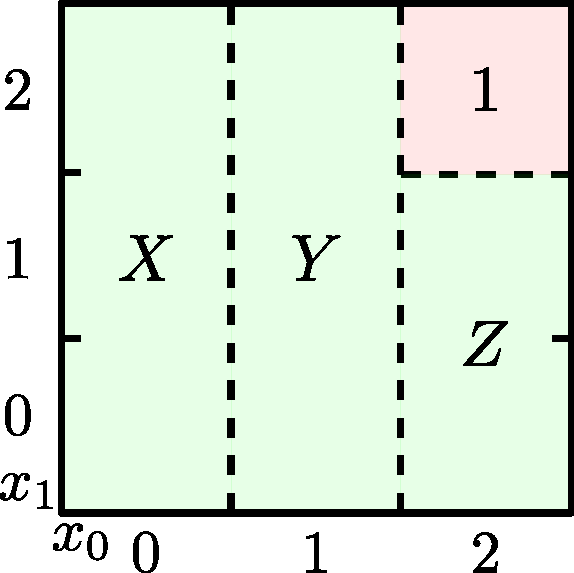
\includegraphics[scale=0.35]{pd_split_thermal.pdf}
    \caption{\textbf{Qutrit phase space regions for $W_{\rho | \tau}(\z)$.}
    Here, the negative component of the magic state overlaps the Wigner distribution of $|0\>$. The rescaled distribution attains a single value in each of the four regions, proportional to the value depicted in the region, see Eq.~(\ref{eq:bmw_rescaled}).
    }
    \label{fig:pd_split}
\end{figure}

We define vectors $\w(\rho), \w(\tau), \w(\rho|\tau)$ based on the values occurring in $W_\rho, W_\tau, W_{\rho|\tau}$ respectively and $\m$ as the vector of associated multiplicities of each value in $W_\rho(\z)$. Specifically, the component values and multiplicities of the relevant distributions in the four distinct regions are given by
\begin{align}
	\m &\coloneqq (1,2,3,3), \\
	\w(\rho) &\coloneqq (-v, u, u, u), \\
	\w(\tau) &\coloneqq \frac{1}{3\Z} \left( e^{-\beta E_0}, e^{-\beta E_0}, e^{-\beta E_1}, e^{-\beta E_2} \right), \\
	\w(\rho | \tau) &\coloneqq 3\Z \left( -v e^{\beta E_0}, u e^{\beta E_0}, u e^{\beta E_1}, u e^{\beta E_2} \right). \label{eq:bmw_rescaled}
\end{align}

Using this notation, the values and multiplicities of the $n$--copy distribution $\w(\rho_n |\tau_n)$ are computed in Proposition~\ref{ncopycomponents}. The values are given by 
\begin{align}\label{eq:ncopy_w_rescaled}
	[\w(\rho_n | \tau_n)]_{ijk} &= (3\Z)^{n} (-v)^{n-\alpha} u^{\alpha} e^{\beta (n-\alpha)E_s} e^{\beta ( i E_0 + j E_1 + k E_2 )},
\end{align}
where the indices $i,j,k$ are non-negative integers that obey the constraint $\alpha \coloneqq i+j+k \leq n$.
The multiplicity of this above value is $m_{ijk}$ with
\begin{equation}
	m_{ijk} = \frac{n!}{i!j!k!(n-\alpha)!} 2^i 3^j 3^k.
\end{equation}
The associated components of $\w(\rho_n)$ are given by
\begin{align}
	[\w(\rho_n)]_{ijk} &= (-v)^{n-\alpha} u^{\alpha}, \label{eq:ncopy_wrho}\\
	[\w(\tau)]_{ijk} &= (3\Z)^{-n} e^{-\beta (n-\alpha)E_s} e^{-\beta ( i E_0 + j E_1 + k E_2 )}. \label{eq:ncopy_wsigma}
\end{align}

In order to construct the $n$--copy Lorenz curve $L_{\rho_n|\tau_n}(x)$ we need to order the components of the distribution, $w(\rho | \tau)_{ijk}$ in decreasing order, and identify the sequence of indices that give us $W_{\rho_n}(\pi(\z))$.

However, in order to obtain a non-trivial bound, it again suffices to use the constraint from the first elbow $(x_0, L_0)$ of $L_{\rho_n|\tau_n}(\z)$. We therefore compute the largest component 
\begin{equation}
	w_{\rm max} \coloneqq \max_{i,j,k} [\w(\rho_n | \tau_n)]_{ijk},
\end{equation}
and determine the indices at which this occurs.
Putting in the values we obtain
\begin{align}
	&(3\Z)^{-n}w_{\rm max} = \nonumber\\
	&\max\limits_{i,j,k}\Big\{ (-v)^{n-\alpha} u^{\alpha} e^{\beta (n-\alpha)E_s} e^{\beta ( i E_0 + j E_1 + k E_2 )} \Big\}, \label{eq:max_slope}
\end{align}
where $0 \leq i,j,k \leq n$ and $\alpha \coloneqq i+j+k \leq n$.
Now for $0 \leq \epsilon \leq 3/7$, we have $v \geq u$. Since we assume that $n$ is even, we need the sum $\alpha = i+j+k$ to be even too, so that the expression is positive. 

Given an even value for $\alpha$, the term $v^{n-\alpha} u^{\alpha} e^{-\beta (n-\alpha)E_s}$ is fixed, so the expression is maximized by setting the coefficient of the highest energy $E_{\rm{max}}$ equal to $\alpha$.
Hence, we have
\begin{align}
	&w_{\rm max} = \nonumber\\
	&(3\Z)^{n} v^n e^{n\beta E_s}\max\limits_{\substack{\alpha = 0,2, \\ \dots,n-2,n}}{\Big\{ \left( \frac{u}{v} e^{\beta (E_{\rm{max}} - E_s)} \right)^{\alpha} \Big\}}.
\end{align}
If the expression $\frac{u(\epsilon)}{v(\epsilon)} e^{\beta (E_{\rm{max}} - E_s)}$ is less than $1$ then the maximum occurs at $\alpha=0$, otherwise it occurs at $\alpha = n$. For a fixed state $\tau$, this transition is determined by the value of the depolarising error parameter $\epsilon$ of the noisy magic state. The transition occurs at $\epsilon = \epsilon_\star$ where
\begin{equation}\label{eq:noise_transition}
	\frac{u(\epsilon_\star)}{v(\epsilon_\star)} e^{\beta (E_{\rm{max}} - E_s)} = \frac{3-\epsilon_\star}{6-8\epsilon_\star} e^{\beta (E_{\rm{max}} - E_s)} = 1.
\end{equation}
If $E_{\rm{max}} = E_s$, namely if the state negativity lies in the same phase space region as the highest energy, this threshold is constant in temperature and given by $\epsilon_{\star} = 3/7$. However, the condition that $\epsilon_\star \ge 0$ also implies a constraint on the effective temperature of the stabilizer state. Specifically, there is a threshold temperature value $\beta_\star$ given by
\begin{equation}
	\beta_{\star} \coloneqq \frac{1}{E_{\rm{max}} - E_s} \ln2,
\end{equation}
such that for the regime $0 \leq \beta \leq \beta_\star$ a threshold error $\epsilon_\star$ exists, and for $\beta > \beta_\star$ no such transition exists, so we choose $\epsilon_\star = 0$. 
Therefore, the transition value for the error is given by
\begin{equation}
	\epsilon_{\star}(\beta) \coloneqq 
	\begin{cases}
		3 - \dfrac{9}{4-2^{\beta/\beta_\star - 1}}, &\text{ for } \beta \leq \beta_\star \\
		0, &\text{ for } \beta > \beta_\star.
	\end{cases}
\end{equation}
The quantity $w(\rho_{\rm{S}} | \sigma)_{\rm{max}}$ is now given by
\begin{equation*}
w_{\rm max} =
	\begin{cases}
		(3\Z)^{n} v^n e^{n\beta E_s}, &\mbox{if }\epsilon \leq \epsilon_{\star},\ \hspace{3pt}\rm{(C1)}\\
		(3\Z)^{n} u^n e^{n\beta E_{\rm{max}}}, &\mbox{if }\epsilon > \epsilon_{\star}.\ \hspace{5pt}\rm{(C2)} 
	\end{cases}
\end{equation*}
Case $\rm{(C1)}$ corresponds to $(i,j,k) = (0,0,0)$, so the multiplicity is $m_{000} = 1$, while
Case $\rm{(C2)}$ corresponds to
\begin{equation}
	(i,j,k) = 
	\begin{cases}
	(0,n,0), &\text{if } E_{\rm{max}} = E_1, \\
	(0,0,n), &\text{if } E_{\rm{max}} = E_2,
	\end{cases}
\end{equation}
so the multiplicity in both cases is $3^n$.

Using that $F = -\beta^{-1} \log \Z$, the first elbow coordinates in the two cases are now given by
\begin{equation}\label{eq:first_elb_coords}
	(x_0, L_0) =
	\begin{cases}
		\left(\frac{1}{3^n} e^{-n\beta (E_s - F)}, v^n \right), &\epsilon \leq \epsilon_\star \vspace{10pt}\\
		\left( e^{-n\beta (E_{\rm{max}}-F)}, (3u)^n \right). &\epsilon > \epsilon_\star
	\end{cases}
\end{equation}

Similarly, considering the output magic state with respect to state $\sigma'$, the image of equilibrium state $\sigma$ under the magic protocol, we get output Lorenz curve coordinates,
\begin{equation}\label{eq:transformed_first_elb_coords}
	(x'_0, L'_0) =
	\begin{cases}
		\left(\frac{1}{3^{n'}} e^{-n\beta (E'_s - F')}, v(\epsilon')^{n'} \right), &\epsilon' \leq \epsilon'_\star \vspace{10pt}\\
		\left( e^{-n'\beta (E'_{\rm{max}}\hspace{-2.5pt}-F')}, (3u(\epsilon'))^{n'} \right), &\epsilon' > \epsilon'_\star
	\end{cases}
\end{equation}
There are four combinations of coordinates, depending on the error parameters $\epsilon, \epsilon'$ for the input and output states.
In each of these combinations, we simply use the first elbow constraint, as described in Proposition~\ref{prop:first_elb}, and manipulate the coordinates as in the proof of Theorem~\ref{thm:free-energy}, leading to the bounds in the statement of this theorem.
\end{proof}

\section*{Supplementary Note 5: Single-shot entropies on quasi-distributions and magic distillation bounds}

In this section, we analyse R\'{e}nyi entropies on quasi-distributions and use them to get magic distillation bounds.

\subsection*{R\'{e}nyi min-divergence from Lorenz curves}
We first demonstrate that the initial slope analysis on the Wigner quasi-distributions makes use of the min-relative divergence. We define 
\begin{equation}
	D_\infty(W_\rho || W_\tau) \coloneqq \log  \max_{\z} \frac{W_\rho(\z)}{W_\tau(\z)},
\end{equation}
which is well-defined since both the nominator and denominator in the above expression are strictly positive when $\tau$ is in the interior of $\F$.

\begin{customthm}{8}
	Let $\tau$ be in the interior of $\F$. Then $D_\infty(W_\rho || W_\tau)$ is well-defined for all $\rho$, and the following hold:
\begin{enumerate}
\item $D_\infty(W_\rho \hspace{1pt}||\hspace{1pt} W_\tau) \ge 0$ for all quantum states $\rho$.
\item  $D_\infty(W_\rho \hspace{1pt}||\hspace{1pt} W_\tau) = 0$ if and only if $\rho =\tau$.
\item $D_\infty(W_{\rho^{\otimes 2n}} \hspace{1pt}||\hspace{1pt} W_{\tau^{\otimes 2n}}) = n D_\infty(W_{\rho^{\otimes 2}} \hspace{1pt}||\hspace{1pt} W_{\tau^{\otimes 2}})$ for any $n \in \mathbb{N}$.
\item $D_\infty(W_\rho \hspace{1pt}||\hspace{1pt} W_\tau) \geq D_\infty(W_{\E(\rho)} \hspace{1pt}||\hspace{1pt} W_{\E(\tau)})$ for any free operation $\E$ such that $\E(\tau)$ is in the interior of $\F$.
\end{enumerate}
\end{customthm}
\begin{proof}
	Since $\tau$ is in the interior of $\F$, its Wigner function obeys $W_\tau(\z) >0$ for all points $\z$ in the phase space. 
In general, $W_\rho(\z)$ is a quasi-distribution, but the given form of $\alpha$ ensures that $W_{\rho}(\z)^\alpha \geq 0$. 
Therefore $D_\infty (W_\rho || W_\tau)$ is always well-defined.

1. We have that 
\begin{equation}
	D_\infty(W_\rho || W_\tau) =\log  \max_{\z} \frac{W_\rho(\z)}{W_\tau(\z)},
\end{equation}
so $2^{D_\infty(W_\rho || W_\tau)}$ equals the slope of the Lorenz curve $L_{\rho|\tau}(x)$ at $x=0$. Since $L_{\rho|\tau}(x)$ is a concave function passing through $(0,0)$ and $(1,1)$ this implies that $L_{\rho |\tau}(x) \ge x$ for all $x \in [0,1]$, and in particular its slope at $x=0$ is always greater than or equal to $1$, which implies $D_\infty(W_\rho || W_\tau) \geq 0$ for all $\rho$.

2. $D_\infty(W_\rho || W_\tau) = 0$ implies that $\max_{\z} \frac{W_\rho(\z)}{W_\tau(\z)}=1$ and the initial slope of $L_{\rho|\tau}(x)$ is $1$. From the concavity of the function and the fact that $L_{\rho|\tau}(1)=1$, this implies that the slope of $L_{\rho|\tau}(x)$ must equal $1$ throughout the interval $[0,1]$ and this, together with the definition of the Lorenz curve, implies that $W_\rho(\z)/W_\tau(\z) = 1$ for all $\z$. Since the Wigner representation $\rho \mapsto W_\rho(\z)$ is bijective this implies that $\rho = \tau$ only. The converse holds by inspection.

3. Given a vector $\w \in \mathbb{R}^N$, it is generally the case that $\max_k w_k \ne \max_k |w_k|$. 
However, we do have that
\begin{equation}
	\max_{k_1,k_2} (w_{k_1} w_{k_2}) = \max_{k_1,k_2} |w_{k_1} w_{k_2}|,
\end{equation}
and if additionally $w_k \geq 0$ for all $k$, then we also have for $2n$ copies that
\begin{equation}
	\max_{k_1, k_2, \dots, k_{2n}} \left( w_{k_1}w_{k_2}\cdots w_{k_{2n}} \right) = (\max_k |w_k|)^{2n},
\end{equation}
and also,
\begin{align}
	&\max_{k_1, k_2, \dots, k_{2n}}\left( w_{k_1}w_{k_2}\cdots w_{k_{2n}} \right) = \nonumber\\
	&\max_{k_1, k_2, \dots, k_{2n}}\left( |w_{k_1}w_{k_2}|\cdots |w_{k_{2n-1}}w_{k_{2n}}| \right) = \nonumber \\
	&\left( \max_{k_1 ,k_2}\left( w_{k_1} w_{k_2} \right) \right)^n.
\end{align}

If we now let $\w = W_{\rho|\tau}(\z) \coloneqq W_{\rho}(\z) /W_{\tau}(\z)$ we have
\begin{equation}
\max_{\z_1, \z_2, \dots ,\z_{2n}} \prod_{k=1}^{2n} W_{\rho|\tau}(\z_k) = \left( \max_{\z_1, \z_2} W_{\rho|\tau}(\z_1)W_{\rho|\tau}(\z_2) \right)^n
\end{equation}
and therefore taking logarithms we have that $D_\infty(W_{\rho^{\otimes 2n}} || W_{\tau^{\otimes 2n}}) = n D_\infty(W_{\rho^{\otimes 2}} || W_{\tau^{\otimes 2}})$ as required.

4. The free operation $\E$ in the Wigner representation corresponds to a stochastic map, which sends $W_\tau(\z)$ to $W_{\E(\tau)}(\z)$, which is another strictly positive probability distribution on the phase space, due to $\E(\tau)$ being in the interior of $\F$. Moreover, $(W_\rho, W_\tau ) \succ (W_{\E(\rho)} , W_{\E(\tau)})$. As shown in the main text this condition holds if and only if $L_{\rho|\tau}(x) \ge L_{\E(\rho)|\E(\tau)}(x)$ for all $x$. In particular, this implies the slope at the origin of the input curve is never less than the slope at the origin of the output curve, and hence the result follows.
\end{proof}

\subsection*{Well-defined R\'{e}nyi entropies on quasi-distributions}

We now make use of known results from majorization theory to establish the Schur-concavity of the R\'{e}nyi entropy $H_\alpha$ on Wigner quasi-distributions for a subset of $\alpha$ values. We consider the set of all quasi-distributions that is a hyper-plane in $\mathbb{R}^N$ given by
\begin{equation}
	\mathcal{Q}_N = \left\{ \w \in \mathbb{R}^N: \sum_{i=1}^N w_i = 1 \right\}.
\end{equation}

We define the notion of \emph{Schur-convex and Schur-convave functions} on a subset $\D \subseteq \mathbb{R}^N$.
\begin{definition} 
	A continuous, real-valued function $f$ defined on $\mathcal{D} \subseteq \mathbb{R}^N$ is called Schur-convex on the domain $\mathcal{D}$ if $\p \prec \q$ on $\mathcal{D}$ implies that $f(\p) \le f(\q)$. A continuous function $f:\mathcal{D} \rightarrow \mathbb{R}$ is called Schur-concave if $(-f)$ is Schur-convex.
\end{definition}
For any subset $\D \subseteq \mathbb{R}^N$ we define
\begin{equation}
	\mathcal{D}^\downarrow \coloneqq \{ \w \in \mathcal{D} : w_1 \ge w_2 \ge \cdots \ge w_N\}.
\end{equation}

We now have the following fundamental result in majorization theory.
\begin{proposition}[Schur-Ostrowski theorem~\cite{Schur_1923, Ostrowski_1952, cit:marshall}] 
	Let $\D\subseteq \mathbb{R}^N$ be a convex set with non-empty interior, and invariant under permutations of vector components. Let $f: \D \rightarrow \mathbb{R}$ be a continuously differentiable function on the interior of $\D$ and continuous on the whole of $\D$. Then $f$ is Schur-convex on $\D$ if and only if $f$ is a symmetric function on $\D$ and 
\begin{equation}
	\partial_1 f(\w) \ge \partial_2 f(\w) \ge \cdots \ge \partial_N f(\w),
\end{equation}
for all $\w$ in the interior of $\mathcal{D}^\downarrow$.
\end{proposition}
Since the set $\mathcal{Q}_N$ of quasi-distributions obey the necessary conditions, we get the following result:
\begin{proposition}
	Let $f$ be a real-valued continuous function defined on $\mathcal{Q}_N$ that is continuously differentiable on the interior of $\mathcal{Q}_N$. 
Then, $f$ is Schur-convex on $\mathcal{Q}_N$ if and only if it is a symmetric function and
\begin{equation}
	\partial_1 f(\w) \ge \partial_2 f(\w) \ge \cdots \ge \partial_N f(\w),
\end{equation}
for all quasi-distributions $\w$ in the interior of $\mathcal{Q}^\downarrow_N$.
\end{proposition}


The classical $\alpha$-R\'{e}nyi entropy on a probability distribution $\p = (p_i)$ is given by
\begin{equation}
	H_\alpha(\p) \coloneqq \frac{1}{1-\alpha} \log \sum_i p_i^\alpha,
\end{equation}
where $\alpha \ge 0$. This means the function is well-defined on $\mathcal{Q}_N^+$, namely the set of quasi-distributions with non-negative components. We wish to extend the domain to the whole of $\mathcal{Q}_N$, but this requires that $w_i^\alpha$ be a real number for any $w_i \in \mathbb{R}$. 

The exponent function $x \mapsto x^\alpha$ is well-defined and real-valued if $\alpha$ is a rational number of the form $\alpha = r / s$ where $s$ is an odd integer and $r \in \mathbb{N}$. However, we also require that $\sum_i w_i^\alpha > 0$ in order for the logarithm to return a real value. To ensure this, we restrict to $\alpha = r/s$ with $r=2a$ being an even integer and $s=2b-1$ being an odd integer, for some integers $a,b\in  \mathbb{N}$, which implies that the following are all well-defined, real-valued expressions,
\begin{equation*}
	0 \le w_i^\alpha = w_i^{\frac{2a}{2b-1}} = \left (w_i^{\frac{1}{2b-1}}\right )^{2a} =\left (w_i^{2a}\right )^{\frac{1}{2b-1}} = |w_i|^{\frac{2a}{2b-1}}.
\end{equation*}
We note that previous work~\cite{Manfredi_2000} has considered the $\alpha=2$ entropy of Wigner distributions, and other work exists that uses the Wehrl entropy, based on the Hussimi function of a quantum state~\cite{Gnutzmann_2001}.

We next show that $H_\alpha (\w)$ for $\alpha = 2a/(2b-1)$ is a Schur-concave function on $\mathcal{Q}_N$ provided that $a \ge b$.
\begin{customthm}{9}\label{thm:HSchur}
	If $\alpha = \frac{2a}{2b-1}$ for positive integers $a,b$ with $a \geq b$, then $H_\alpha(\w)$ is well-defined on the set of quasi-distributions $\mathcal{Q}_N$, and moreover if $\w \succ \w'$ for two quasi-distributions $\w, \w'\in \mathcal{Q}_N$ then $H_\alpha (\w) \leq H_\alpha(\w')$.
\end{customthm}
\begin{proof}
We have $\alpha = \frac{2a}{2b-1} \geq \frac{2b}{2b-1} > 1$ and $\alpha$ is a rational with even numerator and odd denominator, so $\sum_i w_i^\alpha > 0$ and $H_\alpha(\w)$ is well-defined for all quasi-distributions $\w$.

We also have that $H_\alpha(\w)$ is well-defined, continuous, differentiable on the interior of $\mathcal{Q}_N$ and symmetric in the components of $\w$.

Consider the partial derivatives
\begin{equation}
	\frac{\partial H_\alpha}{\partial w_i} = \frac{\alpha}{(\alpha-1)\sum_k{w_k^\alpha}}\left( -w_i^{\alpha-1} \right).
\end{equation}
For $\alpha= \frac{2a}{2b-1}$,  with $a\ge b$, we have that
\begin{equation}
	\frac{\alpha}{(\alpha-1)\sum_k{w_k^\alpha}} > 0.
\end{equation}
The first derivative of the function $g(w) \coloneqq -w^{\alpha - 1}$ is given by
\begin{equation}
	g'(w) = -(\alpha - 1) w^{\alpha-2} = -(\alpha - 1)w^{\frac{2a-4b+2}{2b-1}} \leq 0,
\end{equation}
because $\alpha > 1$ and
\begin{equation}
	w^{\frac{2a-4b+2}{2b-1}} = \left(w^{\frac{a-2b+1}{2b-1}}\right)^{2} \geq 0,
\end{equation}
so $g(w)$ is non-increasing in $w$.

Therefore, whenever $w_i \geq w_j$, we have that 
\begin{equation}
	-w_i^{\alpha-1} \leq -w_j^{\alpha-1},
\end{equation}
which implies that
\begin{equation}
	\frac{\partial H_\alpha}{\partial w_i}(\w) \leq \frac{\partial H_\alpha}{\partial w_j}(\w),
\end{equation}
for any $\w$ in the interior of $\mathcal{Q}_N^\downarrow$.
Therefore, $H_\alpha$ is Schur-concave on $\mathcal{Q}_N$ and
\begin{equation}
	H_\alpha(\w) \leq H_\alpha(\w'),
\end{equation}
for any quasi-distributions $\w, \w'$ that obey $\w \succ \w'$.
\end{proof}
While we have integers $a,b$ such that $0 < \alpha=\frac{2a}{2b-1} < 1$ and $H_\alpha(\w)$ is well-defined, it turns out that monotonicity does not hold if we drop the condition $a \ge b$. If $\alpha =2a/(2b-1)$ with $\alpha < 1$, then $g(w) \coloneqq \frac{-w^{\alpha-1}}{\alpha-1}$ is no longer monotonic for all $w \in \mathbb{R}$, and the problem occurs when comparing $w_i < 0$ and $w_j >0$. As an example of this dependence of monotonicity on the domain of the function, consider the function $g(x) = \frac{1}{x^3}$ which is monotone decreasing on both $x<0$ and $x>0$ separately, however it is not monotone on the full real-line.

We note that if $\alpha =r/s$ with both $r$ and $s$ odd, then $H_\alpha$ is not well-defined for all quasi-distributions, although if the actual set of quasi-distributions has a sufficiently bounded levels negativity, then $\log \sum_{\z} W_\rho(\z)^\alpha$ can still be obtained for $r$ odd, provided the total sum is never negative. This occurs for Wigner distributions, where we have $|W_\rho(\z)| \leq 1/d$ for a $d$--dimensional quantum system.

We also note that the set $F \coloneqq \{2a/(2b-1): a,b \in \mathbb{N} \text{ and } a \geq b\}$ is dense in the reals $\mathbb{R}_{>1}$, as any rational $c/d$ with $c>d$ can be approximated by  $c2^n / (d2^n-1) \in F$ for sufficiently large $n$.

We have that $H_{\alpha}$ is additive on products of quasi-distributions, which we state for completeness.
\begin{proposition}\label{H_add}
	For any $\w \in \mathcal{Q}_N$ and $\w' \in \mathcal{Q}_{N'}$, we have
	\begin{equation}
		H_{\alpha}(\w\otimes \w') = H_{\alpha}(\w) + H_{\alpha}(\w'),
	\end{equation}
	where $\alpha = 2a/(2b-1)$ with positive integers $a\ge b$.
\end{proposition}
\begin{proof}
	\begin{align}
		H_{\alpha}(\w \otimes \w') &= \frac{1}{1-\alpha}\log \sum_{i,j} \left[\w_i \w'_j\right]^{\alpha} \nonumber\\
		&= \frac{1}{1-\alpha}\log  \left [ \sum_i\w_i^\alpha \sum_j\w_j^{\prime \alpha} \right ] \nonumber\\
				&= \frac{1}{1-\alpha}\log  \left [ \sum_i\w_i^\alpha\right ] + \frac{1}{1-\alpha}\log \left [ \sum_j\w_j^{\prime \alpha} \right ] \nonumber\\
		&= H_{\alpha}(\w) + H_{\alpha}(\w').
	\end{align}
\end{proof}

Applied to Wigner distributions $W_\rho (\z)$ for a quantum state $\rho$ we have
\begin{equation}
	H_\alpha(W_\rho) \coloneqq \frac{1}{1-\alpha} \log \sum_{\z} W_{\rho}(\z)^\alpha,
\end{equation}
where $\alpha$ can take values of the form $2a / (2b-1)$, for non-negative integers $a,b$. For the noisy Strange state $\rho = \rho_{\rm{S}}(\epsilon)$, this becomes
\begin{align}
	H_{\alpha}\left(W_{\rho_{\rm{S}}(\epsilon)}\right) = \frac{1}{1-\alpha}\log \left[ 8\left( \frac{1}{6} - \frac{1}{18}\epsilon \right)^\alpha + \left(-\frac{1}{3} + \frac{4}{9}\epsilon \right)^\alpha \right] \nonumber\\
\end{align}
\begin{figure}[t!]
    \centering
    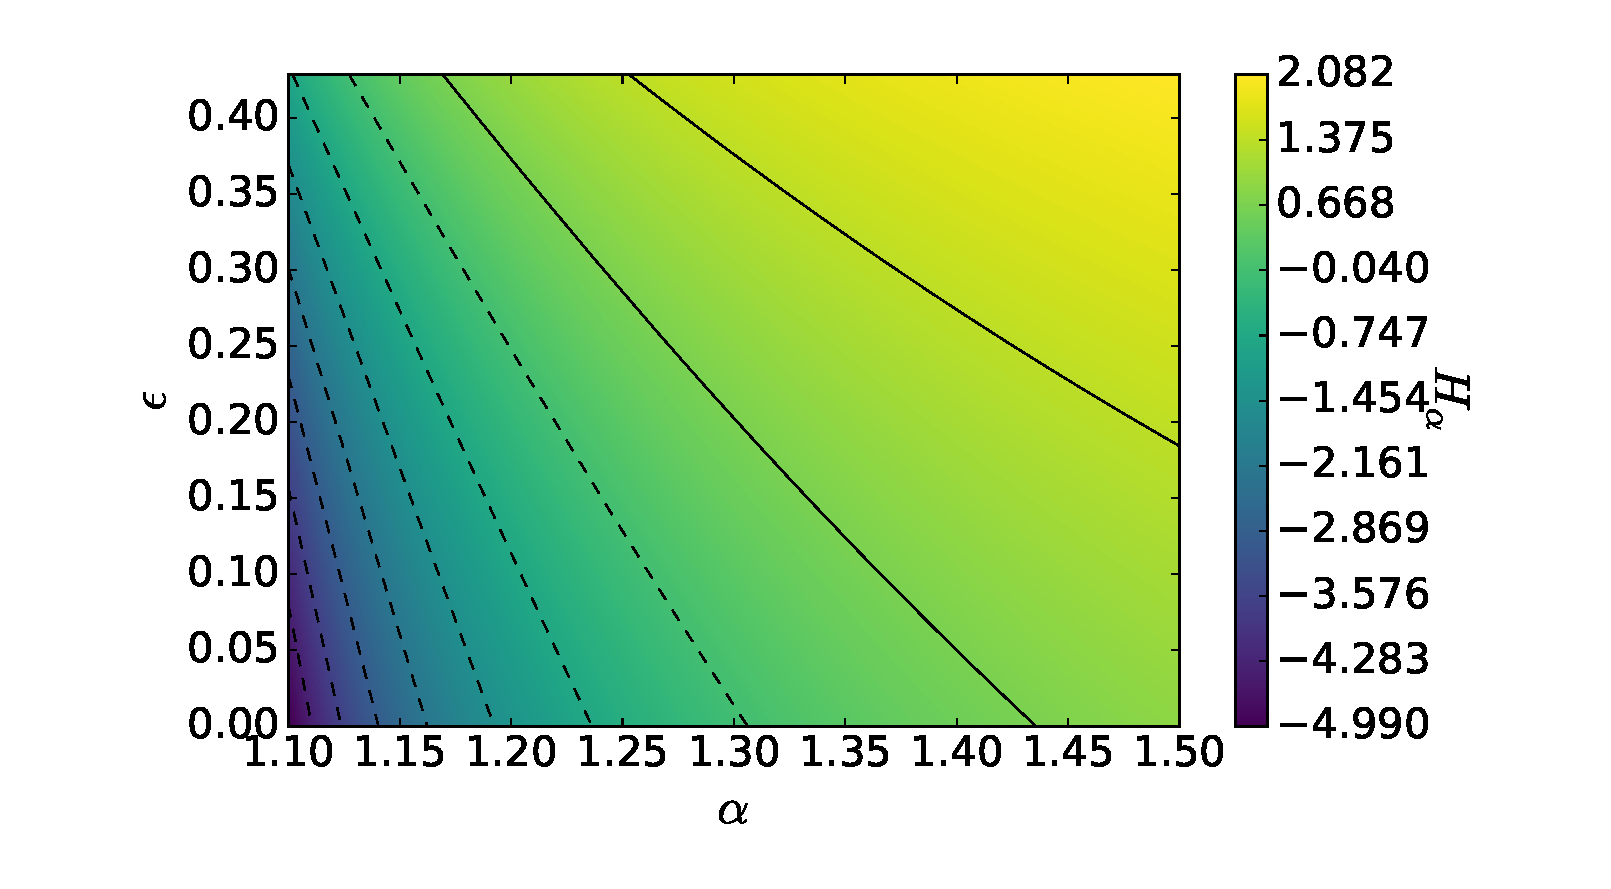
\includegraphics[scale=0.35]{H_vs_eps_a.pdf}
    \caption{\textbf{R\'{e}nyi entropy $H_\alpha$ of the $\epsilon$-noisy Strange state.} $H_\alpha$ is increasing in $\alpha$ and $\epsilon$. The rightmost contour corresponds to $H_\alpha(W_{\rho_{\rm{S}}(\epsilon)}) = 0$. In particular, $H_\alpha(W_{\rho_{\rm{S}}(0)}) = 0$ occurs at $\alpha \approx 1.31$.
    }
    \label{fig:H}
\end{figure}
We now show the following equivalence between Wigner negativity and negative R\'{e}nyi entropies.
\begin{customthm}{10}
	A quantum state $\rho$ has Wigner negativity if and only if $H_\alpha(W_\rho) < 0$ for some $\alpha =  \frac{2a}{2b-1}$, with positive integers $a \geq b$.
\end{customthm}
\begin{proof} 
If we have $H_\alpha (W_\rho) <0 $ for $\alpha >1$, then it follows that $\log \sum_{\z} W_\rho (\z)^\alpha > 1$. 
However, it is known that $H_\alpha$ is always non-negative on probability distributions, so $W_\rho(\z)$ must be a strict quasi-distribution with negativity.

Conversely, suppose $\rho$ has negativity in its Wigner representation. This in particular implies that $\sum_{\z} |W_\rho (\z)| >1$. We now consider $\sum_{\z} W_\rho (\z)^{\frac{2a}{2b-1}}$ for positive integers $a\ge b$. We have that
\begin{align}
\sum_{\z} W_\rho (\z)^{\frac{2a}{2b-1}} &= \sum_{\z} |W_\rho (\z)|^{\frac{2a}{2b-1}} \nonumber \\
&= \sum_{\z} |W_\rho (\z)|^{1+ \epsilon},
\end{align}
where $\epsilon = \alpha -1=\frac{2a}{2b-1} - 1 >0$. By choosing the positive integers $a$ and $b$ sufficiently large we can make $\epsilon$ arbitrarily close to $0$. This implies that there exists a sequence $\epsilon_n= \alpha_n-1 =\frac{2a_n}{2b_n-1} - 1$ with integer pairs $a_n, b_n$ such that
\begin{equation}
\sum_{\z} |W_\rho (\z)|^{1+ \epsilon_n} \rightarrow \sum_{\z} |W_\rho (\z)| >1,
\end{equation}
as $n$ increases.
Since $\frac{1}{1-\alpha_n} <0$ for any $n$ it follows that $H_{\alpha_n} (W_\rho) = \frac{1}{1-\alpha_n} \log \sum_{\z} W_\rho (\z)^{\alpha_n}  <0 $ at some point in the sequence, which completes the proof.
\end{proof}
Therefore Wigner negativity coincides with negativity of a R\'{e}nyi entropy.

\subsection*{R\'{e}nyi divergences on quasi-distributions}
We now define the $\alpha$-R\'{e}nyi divergence for a quasi-distribution $\w \in \mathcal{Q}_N$ relative to a full-rank probability distribution $\r\in \mathcal{Q}_N^+$ as
\begin{equation}
	D_\alpha(\w||\r) \coloneqq \frac{1}{\alpha - 1} \log \sum_{i} w_i^\alpha r_i^{1-\alpha},
\end{equation}
where $\alpha=2a/(2b-1)$ for positive integers $a \ge b$. We now have the following result that relates the R\'{e}nyi divergence to the R\'{e}nyi entropy on a dense subset of probability distributions.
\begin{proposition}\label{H2D}
	Let $\w\in \mathcal{Q}_N$ be a quasi-distribution and $\r \in \mathcal{Q}_N^+$ a probability distribution with positive rational entries given by $r_i = a_i/K$ for positive integers $a_i$ and $K = \sum_{i=1}^N a_i$.
	Then,
	\begin{equation}
		H_\alpha(\Gamma_{\bma}(\w)) = K - D_\alpha(\w \hspace{1pt}||\hspace{1pt} \r),
	\end{equation}
	where $\alpha = 2a / (2b-1)$ for positive integers $a \ge b$.
\end{proposition}
\begin{proof}
	For the given form of $\alpha$ and positive $r_i,\ i=1,\dots,N$, $D_\alpha(\w || \r)$ is well-defined for all $\w$. From the definition of $\Gamma_{\bma}$ we have
	\begin{equation}
		\Gamma_{\bma}(\w) = \bigoplus_{i=1}^N w_i (1/a_i, 1/a_i, \dots, 1/a_i).
	\end{equation}
	This directly leads to
	\begin{align}
		H_\alpha(\Gamma_{\bma}(\w)) &= \frac{1}{1-\alpha} \log \sum_{i=1}^N a_i \left( \frac{w_i}{a_i} \right)^\alpha \nonumber\\
		&= \frac{1}{1-\alpha} \log \sum_{i=1}^N w_i^{\alpha} a_i^{1-\alpha} \nonumber\\
		&= \frac{1}{1-\alpha} \log K^{1-\alpha} \sum_{i=1}^N w_i^{\alpha} r_i^{1-\alpha} \nonumber\\
		&= K + \frac{1}{1-\alpha} \log \sum_{i=1}^N w_i^{\alpha} r_i^{1-\alpha} \nonumber\\
		&= K - D_\alpha(\w ||\r).
	\end{align}
\end{proof}
With this we now establish monotonicity for R\'{e}nyi relative divergences.
\begin{proposition}\label{DSchur}
	Let $\alpha = \frac{2a}{2b-1}$ for any positive integers $a,b$ with $a \geq b$. Let $\w \in \mathcal{Q}_N$, $\w' \in \mathcal{Q}_{N'}$ and $\r \in  \mathcal{Q}^+_N$, $\r' \in \mathcal{Q}^+_{N'}$ with positive rational components $a_i/K$ and $a'_i/K$ respectively.
	Then $D_\alpha(\w \hspace{1pt}||\hspace{1pt} \r) \geq D_\alpha(\w' \hspace{1pt}||\hspace{1pt} \r')$, whenever $(\w, \r) \succ (\w', \r')$.
\end{proposition}
\begin{proof}
	The statement $(\w, \r) \succ (\w', \r')$ is equivalent to $\Gamma_{\bma}(\w) \succ \Gamma_{\bma'}(\w')$.
	Therefore, due to Theorem~\ref{thm:HSchur} we have
	\begin{equation}
		H_\alpha(\Gamma_{\bma}(\w)) \leq H_\alpha(\Gamma_{\bma'}(\w'))
	\end{equation}
	which, due to Proposition~\ref{H2D}, is equivalent to
	\begin{equation}
		D_\alpha(\w \hspace{1pt}||\hspace{1pt} \r) \geq D_\alpha(\w' \hspace{1pt}||\hspace{1pt} \r').
	\end{equation}
\end{proof}
Since the rationals are dense in the real numbers we can assume any Wigner distribution considered has rational components without affecting results.
We now specialize to Wigner distributions of quantum states, and quantum operations that map the set of free states $\F$ into itself.
\begin{customthm}{11}\label{thm:Da_props}
	Let $\tau$ be in the interior of $\F$. 
	If $\alpha = \frac{2a}{2b-1}$ for positive integers $a,b$ with $a \geq b$, then the $\alpha$-R\'{e}nyi divergence $D_\alpha(W_\rho \hspace{1pt}||\hspace{1pt} W_\tau)$ is well-defined for all states $\rho$, and the following hold:
\begin{enumerate}
\item $D_\alpha(W_\rho \hspace{1pt}||\hspace{1pt} W_\tau) \ge 0$ for all quantum states $\rho$.
\item  $D_\alpha(W_\rho \hspace{1pt}||\hspace{1pt} W_\tau) = 0$ if and only if $\rho =\tau$.
\item $D_\alpha(W_{\rho^{\otimes n}} \hspace{1pt}||\hspace{1pt} W_{\tau^{\otimes n}}) = n D_\alpha(W_\rho \hspace{1pt}||\hspace{1pt} W_\tau)$ for any $n \in \mathbb{N}$.
\item $D_\alpha(W_\rho \hspace{1pt}||\hspace{1pt} W_\tau) \geq D_\alpha (W_{\E(\rho)} \hspace{1pt}||\hspace{1pt} W_{\E(\tau)})$ for any free operation $\E$ such that $\E(\tau)$ is in the interior of $\F$.
\end{enumerate}
\end{customthm}
\begin{proof}
	Since $\tau$ is in the interior of $\F$, its Wigner function obeys $W_\tau(\z) >0$ for all points $\z$ in the phase space. 
In general, $W_\rho(\z)$ is a quasi-distribution, but for $\alpha = 2a/2b-1$ we that $W_{\rho}(\z)^\alpha \geq 0$. 
Therefore $D_\alpha (W_\rho || W_\tau)$ is always well-defined and real-valued.

1. $D_\alpha$ is Schur-convex and every pair $(W_{\rho}, W_{\tau})$ majorizes the pair $(W_{\id/d}, W_{\id/d})$, so
\begin{align}
	D_\alpha(W_{\rho} \hspace{1pt}||\hspace{1pt} W_{\tau}) \geq D_\alpha(W_{\id/d} \hspace{1pt}||\hspace{1pt} W_{\id/d}) &= \nonumber\\
	\frac{1}{\alpha-1} \log \sum_{\z} W_{\id/d}(\z) &= 0.
\end{align}

2. In the inequality of property 1, equality holds iff $L_{\rho|\tau}(x) = L_{\id/d|\id/d}(x) = L_{\tau|\tau}(x)$ for all $x\in [0,1]$ due to Proposition~\ref{prop:rmajor} which in turn holds iff $\rho = \tau$.

3. This property follows from the multiplicativity of the Wigner distribution.
In particular,
\begin{align}
	&D_\alpha(W_{\rho^{\otimes n}} \hspace{1pt}||\hspace{1pt} W_{\tau^{\otimes n}}) = \nonumber\\
	&\frac{1}{\alpha - 1} \log \sum_{\z} W_{\rho^{\otimes n}}(\z)^\alpha W_{\tau^{\otimes n}}(\z)^{1-\alpha} = \nonumber\\
	&\frac{1}{\alpha - 1} \log \sum_{\z} \prod_{i=1}^n W_{\rho}(\z_i)^\alpha W_{\tau}(\z_i)^{1-\alpha} = \nonumber\\
	&\frac{1}{\alpha - 1} \log \prod_{i=1}^n \sum_{\z_i} W_{\rho}(\z_i)^\alpha W_{\tau}(\z_i)^{1-\alpha} = \nonumber\\
	&\sum_{i=1}^n \frac{1}{\alpha - 1} \log \sum_{\z'} W_{\rho}(\z')^\alpha W_{\tau}(\z')^{1-\alpha} = \nonumber\\
	&= n D_{\alpha}(W_\rho \hspace{1pt}||\hspace{1pt} W_\tau).
\end{align}

4. This follows immediately from the fact that $(W_\rho, W_\tau) \succ (W_{\E(\rho)}, W_{\E(\tau)})$ for any free quantum channel $\E$ that sends $\tau$ into the interior of $\F$, and the Schur-convexity of $D_\alpha$.
\end{proof}

We are now in a position to derive general magic state distillation bounds.
\begin{customthm}{12}
	Consider a general magic state distillation protocol on odd prime dimension qudits, that converts a magic state $\rho^{\otimes n} \longrightarrow \E(\rho^{\otimes n})=\rho'^{\otimes m}$ and let $\tau$ be any full-rank stabilizer reference state on a qudit. Then, the distillation rate $R \coloneqq m/n$ is upper bounded as
	\begin{equation}
		R \leq R_\alpha \coloneqq \frac{D_{\alpha}(W_\rho \hspace{1pt}||\hspace{1pt} W_\tau)}{\rlap{\raisebox{-0.2ex}{$\widetilde{\phantom{D}}$}}D_\alpha( \rho', \tau')},
	\end{equation}
	where $\alpha = \frac{2a}{2b-1}$ for any positive integers $a,b$ with $a \geq b$ and the average divergence per qudit
	\begin{equation}
\widetilde{D}_\alpha( \rho', \tau') \coloneqq \frac{1}{m} D_\alpha (W_{\rho'^{\otimes m}} \hspace{1pt}||\hspace{1pt} W_{\tau'_m}),
\end{equation}
between the output magic state $\rho'^{\otimes m}$ and $\tau'_m = \E(\tau^{\otimes n})$.
\end{customthm}
\begin{proof}
	The bound is a direct consequence of the properties of the $\alpha$--R\'{e}nyi divergence in Theorem~\ref{thm:Da_props}.
	
Due to the action of the magic protocol channel, we get
\begin{equation}	
	D_\alpha(W_{\rho^{\otimes n}} \hspace{1pt}||\hspace{1pt} W_{\tau^{\otimes n}}) \geq D_\alpha (W_{\rho'^{\otimes m}} \hspace{1pt}||\hspace{1pt} W_{\tau'_m}).\vspace{10pt}
\end{equation}

We can use the additivity to rewrite this as
\begin{equation}
	n D_\alpha(W_\rho \hspace{1pt}||\hspace{1pt} W_\tau) \geq m \frac{1}{m}D_\alpha(W_{\rho'^{\otimes m}} \hspace{1pt}||\hspace{1pt} W_{\tau'_m}).
\end{equation}

Since $\rho'^{\otimes m} \neq \tau'_m$, we have $D_\alpha(W_{\rho'^{\otimes m}} \hspace{1pt}||\hspace{1pt} W_{\tau'_m}) > 0$, which directly leads to the bound
\begin{equation}
	\frac{m}{n} \leq \frac{D_{\alpha}(W_\rho \hspace{1pt}||\hspace{1pt} W_\tau)}{\rlap{\raisebox{-0.1ex}{$\widetilde{\phantom{D}}$}}D_\alpha( \rho', \tau')}.
\end{equation}
\end{proof}

\onecolumngrid

\section*{Supplementary References}
\vspace{-12pt}

\providecommand{\noopsort}[1]{}\providecommand{\singleletter}[1]{#1}
\begin{thebibliography}{10}
\expandafter\ifx\csname url\endcsname\relax
  \def\url#1{\texttt{#1}}\fi
\expandafter\ifx\csname urlprefix\endcsname\relax\def\urlprefix{}\fi
\providecommand{\bibinfo}[2]{#2}
\providecommand{\eprint}[2][]{\url{#2}}

\bibitem{cit:veitch}
\bibinfo{author}{Veitch, V.}, \bibinfo{author}{Ferrie, C.},
  \bibinfo{author}{Gross, D.} \& \bibinfo{author}{Emerson, J.}
\newblock \bibinfo{title}{Negative quasi-probability as a resource for quantum
  computation}.
\newblock \emph{\bibinfo{journal}{New Journal of Physics}}
  \textbf{\bibinfo{volume}{14}}, \bibinfo{pages}{113011}
  (\bibinfo{year}{2012}).
\newblock \urlprefix\url{https://doi.org/10.1088/1367-2630/14/11/113011}.

\bibitem{Vourdas_2004}
\bibinfo{author}{Vourdas, A.}
\newblock \bibinfo{title}{Quantum systems with finite hilbert space}.
\newblock \emph{\bibinfo{journal}{Reports on Progress in Physics}}
  \textbf{\bibinfo{volume}{67}}, \bibinfo{pages}{267--320}
  (\bibinfo{year}{2004}).
\newblock \urlprefix\url{https://doi.org/10.1088/0034-4885/67/3/r03}.

\bibitem{Gross2006}
\bibinfo{author}{Gross, D.}
\newblock \bibinfo{title}{Hudson’s theorem for finite-dimensional quantum
  systems}.
\newblock \emph{\bibinfo{journal}{Journal of Mathematical Physics}}
  \textbf{\bibinfo{volume}{47}}, \bibinfo{pages}{122107}
  (\bibinfo{year}{2006}).
\newblock \urlprefix\url{https://aip.scitation.org/doi/10.1063/1.2393152}.

\bibitem{Wang_2019}
\bibinfo{author}{Wang, X.}, \bibinfo{author}{Wilde, M.~M.} \&
  \bibinfo{author}{Su, Y.}
\newblock \bibinfo{title}{Quantifying the magic of quantum channels}.
\newblock \emph{\bibinfo{journal}{New Journal of Physics}}
  \textbf{\bibinfo{volume}{21}}, \bibinfo{pages}{103002}
  (\bibinfo{year}{2019}).
\newblock \urlprefix\url{https://doi.org/10.1088/1367-2630/ab451d}.

\bibitem{cit:mirsky}
\bibinfo{author}{Mirsky, L.}
\newblock \bibinfo{title}{On the trace of matrix products}.
\newblock \emph{\bibinfo{journal}{Mathematische Nachrichten}}
  \textbf{\bibinfo{volume}{20}}, \bibinfo{pages}{171--174}
  (\bibinfo{year}{1959}).
\newblock
  \urlprefix\url{https://onlinelibrary.wiley.com/doi/abs/10.1002/mana.19590200306}.

\bibitem{cit:horodecki2013}
\bibinfo{author}{Horodecki, M.} \& \bibinfo{author}{Oppenheim, J.}
\newblock \bibinfo{title}{Fundamental limitations for quantum and nanoscale
  thermodynamics}.
\newblock \emph{\bibinfo{journal}{Nature Communications}}
  \textbf{\bibinfo{volume}{4}}, \bibinfo{pages}{2059} (\bibinfo{year}{2013}).
\newblock \urlprefix\url{https://doi.org/10.1038/ncomms3059}.

\bibitem{Brandao_2015}
\bibinfo{author}{Brand{\~a}o, F.}, \bibinfo{author}{Horodecki, M.},
  \bibinfo{author}{Ng, N.}, \bibinfo{author}{Oppenheim, J.} \&
  \bibinfo{author}{Wehner, S.}
\newblock \bibinfo{title}{The second laws of quantum thermodynamics}.
\newblock \emph{\bibinfo{journal}{Proceedings of the National Academy of
  Sciences}} \textbf{\bibinfo{volume}{112}}, \bibinfo{pages}{3275--3279}
  (\bibinfo{year}{2015}).
\newblock \urlprefix\url{https://www.pnas.org/content/112/11/3275}.

\bibitem{cit:lostaglio}
\bibinfo{author}{Lostaglio, M.}
\newblock \bibinfo{title}{An introductory review of the resource theory
  approach to thermodynamics}.
\newblock \emph{\bibinfo{journal}{Reports on Progress in Physics}}
  \textbf{\bibinfo{volume}{82}}, \bibinfo{pages}{114001}
  (\bibinfo{year}{2019}).
\newblock \urlprefix\url{https://doi.org/10.1088/1361-6633/ab46e5}.

\bibitem{cit:marshall}
\bibinfo{author}{Marshall, A.~W.}, \bibinfo{author}{Olkin, I.} \&
  \bibinfo{author}{Arnold, B.~C.}
\newblock \emph{\bibinfo{title}{Inequalities: Theory of Majorization and Its
  Applications}} (\bibinfo{publisher}{Springer}, \bibinfo{year}{2011}).

\bibitem{ruch_mixing_1978}
\bibinfo{author}{Ruch, E.}, \bibinfo{author}{Schranner, R.} \&
  \bibinfo{author}{Seligman, T.~H.}
\newblock \bibinfo{title}{The mixing distance}.
\newblock \emph{\bibinfo{journal}{The Journal of Chemical Physics}}
  \textbf{\bibinfo{volume}{69}}, \bibinfo{pages}{386--392}
  (\bibinfo{year}{1978}).
\newblock \urlprefix\url{https://aip.scitation.org/doi/10.1063/1.436364}.

\bibitem{Renes_2016}
\bibinfo{author}{Renes, J.~M.}
\newblock \bibinfo{title}{Relative submajorization and its use in quantum
  resource theories}.
\newblock \emph{\bibinfo{journal}{Journal of Mathematical Physics}}
  \textbf{\bibinfo{volume}{57}}, \bibinfo{pages}{122202}
  (\bibinfo{year}{2016}).
\newblock \urlprefix\url{https://aip.scitation.org/doi/10.1063/1.4972295}.

\bibitem{Buscemi_2017}
\bibinfo{author}{Buscemi, F.} \& \bibinfo{author}{Gour, G.}
\newblock \bibinfo{title}{Quantum relative lorenz curves}.
\newblock \emph{\bibinfo{journal}{Phys. Rev. A}} \textbf{\bibinfo{volume}{95}},
  \bibinfo{pages}{012110} (\bibinfo{year}{2017}).
\newblock \urlprefix\url{https://link.aps.org/doi/10.1103/PhysRevA.95.012110}.

\bibitem{cit:ash}
\bibinfo{author}{Ash, R.}
\newblock \emph{\bibinfo{title}{Information Theory}} (\bibinfo{publisher}{Dover
  Publications Inc.}, \bibinfo{year}{1965}).
\newblock
  \urlprefix\url{https://www.semanticscholar.org/paper/Information-Theory-Ash/e9f30be9279c6000ce5602370950748cc2c79101}.

\bibitem{Schur_1923}
\bibinfo{author}{Schur, I.}
\newblock \bibinfo{title}{{\"U}ber eine klasse von mittelbildungen mit
  anwendungen auf die determinantentheorie}.
\newblock \emph{\bibinfo{journal}{Berliner Mathematische Gesellschaft}}
  \textbf{\bibinfo{volume}{22}}, \bibinfo{pages}{9--20} (\bibinfo{year}{1923}).

\bibitem{Ostrowski_1952}
\bibinfo{author}{Ostrowski, A.~M.}
\newblock \bibinfo{title}{Sur quelques applications des fonctions convexes et
  concaves au sens de i. schur}.
\newblock \emph{\bibinfo{journal}{Journal de Mathématiques Pures et
  Appliquées}} \textbf{\bibinfo{volume}{31}}, \bibinfo{pages}{253--292}
  (\bibinfo{year}{1952}).

\bibitem{Manfredi_2000}
\bibinfo{author}{Manfredi, G.} \& \bibinfo{author}{Feix, M.~R.}
\newblock \bibinfo{title}{Entropy and {W}igner functions}.
\newblock \emph{\bibinfo{journal}{Phys. Rev. E}} \textbf{\bibinfo{volume}{62}},
  \bibinfo{pages}{4665--4674} (\bibinfo{year}{2000}).
\newblock \urlprefix\url{https://link.aps.org/doi/10.1103/PhysRevE.62.4665}.

\bibitem{Gnutzmann_2001}
\bibinfo{author}{Gnutzmann, S.} \& \bibinfo{author}{{\.{Z}}yczkowski, K.}
\newblock \bibinfo{title}{R{\'{e}}nyi-wehrl entropies as measures of
  localization in phase space}.
\newblock \emph{\bibinfo{journal}{Journal of Physics A: Mathematical and
  General}} \textbf{\bibinfo{volume}{34}}, \bibinfo{pages}{10123--10139}
  (\bibinfo{year}{2001}).
\newblock \urlprefix\url{https://doi.org/10.1088/0305-4470/34/47/317}.

\end{thebibliography}


\end{document}